% =============================================================================
%  Two-Timescale Secure Transmission for MA-Enabled Multiuser Systems
%  With Statistical Eavesdropper CSI
%  Compile with pdfLaTeX and the official IEEEtran.cls (TeX Live / Overleaf).
% =============================================================================
\documentclass[journal]{IEEEtran}
\usepackage{amsmath,amssymb,amsfonts}
\interdisplaylinepenalty=2500
\usepackage{algorithm}
\usepackage{algpseudocode}
\usepackage{cite}
\usepackage{graphicx}
\usepackage[caption=false,font=footnotesize]{subfig}
\graphicspath{{ma_secrecy_matlab/results/}}
\usepackage{tikz}
\usetikzlibrary{arrows.meta,decorations.pathreplacing,calc}

% ------------------------------- theorem-like --------------------------------
\newtheorem{lemma}{Lemma}
\newtheorem{proposition}{Proposition}
\newcounter{remarkctr}
\newcommand{\remarkhead}[1]{\refstepcounter{remarkctr}\textit{Remark~\theremarkctr\ (#1):}}

% ----------------------------- notation macros -------------------------------
\newcommand{\E}{\mathbb{E}}
\newcommand{\CN}{\mathcal{CN}}
\newcommand{\tr}{\mathrm{tr}}
\newcommand{\diag}{\mathrm{diag}}
\newcommand{\RE}{\mathrm{Re}}
\newcommand{\bt}{\mathbf{t}}
\newcommand{\bh}{\mathbf{h}}
\newcommand{\bg}{\mathbf{g}}
\newcommand{\hb}{\bar{\mathbf{h}}}
\newcommand{\gb}{\bar{\mathbf{g}}}
\newcommand{\htl}{\tilde{\mathbf{h}}}
\newcommand{\gtl}{\tilde{\mathbf{g}}}
\newcommand{\bH}{\mathbf{H}}
\newcommand{\Hb}{\bar{\mathbf{H}}}
\newcommand{\Htl}{\tilde{\mathbf{H}}}
\newcommand{\bK}{\mathbf{K}}
\newcommand{\bB}{\mathbf{B}}
\newcommand{\bL}{\mathbf{L}}
\newcommand{\bI}{\mathbf{I}}
\newcommand{\bw}{\mathbf{w}}
\newcommand{\wb}{\bar{\mathbf{w}}}
\newcommand{\bv}{\mathbf{v}}
\newcommand{\bp}{\mathbf{p}}
\newcommand{\ba}{\mathbf{a}}
\newcommand{\be}{\mathbf{e}}
\newcommand{\bb}{\mathbf{b}}
\newcommand{\bl}{\mathbf{l}}
\newcommand{\br}{\mathbf{r}}
\newcommand{\bx}{\mathbf{x}}
\newcommand{\bz}{\mathbf{z}}
\newcommand{\bF}{\mathbf{F}}
\newcommand{\Fb}{\bar{\mathbf{F}}}
\newcommand{\bW}{\mathbf{W}}
\newcommand{\bD}{\mathbf{D}}
\newcommand{\bX}{\mathbf{X}}
\newcommand{\bOm}{\boldsymbol{\Omega}}
\newcommand{\bPhi}{\boldsymbol{\Phi}}
\newcommand{\bGam}{\boldsymbol{\Gamma}}
\newcommand{\bSig}{\boldsymbol{\Sigma}}
\newcommand{\bDel}{\boldsymbol{\Delta}}
\newcommand{\bPi}{\boldsymbol{\Pi}}
\newcommand{\Ptot}{P_{\mathrm{tot}}}
\newcommand{\Dmin}{D_{\min}}
\newcommand{\sbe}{\bar{\sigma}_e^2}
\newcommand{\PHp}{\mathbf{P}_{\mathbf{H}}^{\perp}}
\newcommand{\PH}{\mathbf{P}_{\mathbf{H}}}

\begin{document}

\title{Two-Timescale Secure Transmission for Movable Antenna-Enabled Multiuser Systems With Statistical Eavesdropper CSI}

\author{Author~One,~\IEEEmembership{Student Member,~IEEE,}
        Author~Two,~\IEEEmembership{Member,~IEEE}
\thanks{The authors are with ... (e-mail: ...).}}

\markboth{IEEE Transactions on Communications (draft)}{}

\maketitle

\begin{abstract}
Movable antennas (MAs) can reshape the spatial correlation between the channels of legitimate users (LUs) and an eavesdropper (Eve), providing a new degree of freedom for physical layer security. However, existing MA-aided secure designs mostly rely on instantaneous channel state information (CSI), which is hindered by the movement delay, the overhead of acquiring the CSI over the movable region, and the unavailability of the instantaneous CSI of a passive Eve. We propose a two-timescale secure transmission framework for an MA-enabled multiuser downlink system, where the antenna positions and the power allocation between the confidential signals and artificial noise (AN) are optimized based on statistical CSI, whereas zero-forcing precoding and null-space AN are designed based on the instantaneous CSI of the LUs only. We prove that the information leakage and the AN received by Eve are conditionally independent given the channels of the LUs, and derive a closed-form approximation of the ergodic wiretap rate. The resulting approximate ergodic secrecy sum rate (ESSR) depends on the antenna positions only through three geometric quantities. We then develop an alternating optimization algorithm, where the power allocation admits a secrecy water-filling structure and the antenna positions are updated via majorization--minimization. Numerical results show that, at a transmit signal-to-noise ratio of $20$~dB, the proposed design improves the ESSR by $12.5\%$ and $27.1\%$ over the rate-oriented two-timescale MA design and a fixed-position array, respectively, outperforms antenna selection with twice as many antennas, enhances secrecy even for a single LU, and reduces the required AN power.
\end{abstract}

\begin{IEEEkeywords}
Movable antenna, physical layer security, artificial noise, two-timescale design, statistical CSI, ergodic secrecy rate.
\end{IEEEkeywords}

\IEEEpeerreviewmaketitle

% =============================================================================
\section{Introduction}
% =============================================================================
\IEEEPARstart{P}{hysical} layer security (PLS) exploits the randomness and the spatial characteristics of wireless channels to protect confidential messages against eavesdropping, which complements upper-layer cryptography~\cite{Wyner1975,Mukherjee2014,WuJSAC2018}. In multi-antenna systems, secure precoding and artificial noise (AN) are two main enablers of PLS~\cite{Goel2008,Zhou2010}, whose performance is fundamentally limited by how well the legitimate users (LUs) and the eavesdropper (Eve) can be spatially separated. When Eve is located in a direction close to that of an LU and the line-of-sight (LoS) propagation is dominant, their channels are highly correlated, and a conventional fixed-position antenna (FPA) array can hardly steer the information-bearing beams away from Eve without sacrificing the beamforming gain at the LU.

Movable antennas (MAs), also known as fluid antennas, have recently emerged as a promising technology to overcome this limitation~\cite{ZhuMag2024,ZhuTWC2024Model,WongTWC2021}. By adjusting the antenna positions within a given region, MAs reshape the channel correlation among different receivers without additional radio-frequency (RF) chains~\cite{MaTWC2024,ZhuTWC2024MU,ZhuCL2023}, which can be exploited to decorrelate the channels of the LUs from that of Eve. The authors of~\cite{HuSPL2024} jointly optimized the transmit beamforming and the positions of an MA array to maximize the secrecy rate with perfect channel state information (CSI), and the statistical CSI of the eavesdroppers was exploited in~\cite{HuTMC2024} when their instantaneous CSI is unavailable. More recently, a deterministic equivalent of the ergodic secrecy rate of a multiple-input multiple-output multiple-eavesdropper-antenna MA system with partial CSI of Eve was derived in~\cite{XieArxiv2026}, and a sensing-assisted secure design was developed in~\cite{ChenArxiv2026}, where the MA positions enhance both the estimation of the direction of Eve and the secrecy rate.

However, the above works optimize the antenna positions based on the instantaneous CSI of at least the LUs, which requires the antennas to be repositioned in each channel coherence interval (CI) under fast fading. Such single-timescale designs are difficult to implement, since the mechanical movement incurs non-negligible delay and energy consumption, the CSI is required over the entire movable region, which, under Rician fading, can only be acquired by traversing the region~\cite{ZhengTCOM2025,HuTVT2025}, and the instantaneous CSI of a passive Eve is generally unavailable. To reduce the overhead, two-timescale MA designs have been proposed~\cite{ZhengTCOM2025,HuTVT2025}, following the paradigm developed for intelligent reflecting surfaces~\cite{ZhaoTWC2021}, where the antenna positions are optimized based on the statistical CSI, and the beamforming is designed based on the instantaneous CSI of the resulting effective channels. However, these works focused on the ergodic sum rate, and the two-timescale design of MA-enabled secure transmission has not been investigated yet.

Extending the two-timescale MA design to secure transmission is not straightforward. First, the ergodic wiretap rate of Eve is determined by the random precoding directions and AN subspace induced by the instantaneous CSI of the LUs, whereas the existing ergodic-rate approximations for zero-forcing (ZF) precoding~\cite{ZhangJSTSP2014,ZhengTCOM2025,HuTVT2025} only characterize the signal power received by the intended users. Second, in the rate-oriented design, the antenna positions improve the ergodic rate only by decorrelating the users, and thus bring no gain for a single user~\cite{ZhengTCOM2025}, whereas in secure transmission they also determine the information leakage and the AN received by Eve. Third, the power allocation between the confidential signals and the AN is coupled with the antenna positions. The main contributions of this paper are summarized as follows.
\begin{itemize}
\item We propose a two-timescale secure transmission framework for MA-enabled multiuser systems, where the antenna positions and the long-term power allocation among the confidential signals and AN are optimized based on the statistical CSI of the LUs and Eve, and ZF precoding and null-space AN are designed based on the instantaneous CSI of the LUs only. It requires neither the instantaneous CSI of Eve nor frequent antenna movement.
\item We prove that the information leakage and the AN received by Eve are conditionally independent given the channels of the LUs, and derive a closed-form approximation of the ergodic wiretap rate, which is exact in the non-LoS (NLoS)-dominant regime and asymptotically exact in the LoS-dominant regime. The resulting approximate ergodic secrecy sum rate (ESSR) depends on the antenna positions only through three geometric quantities, which reveals that the MAs enhance secrecy by decorrelating the LUs, reducing the information leakage, and increasing the AN received by Eve, even for a single LU.
\item We develop an alternating optimization (AO) algorithm to maximize the ESSR, where the power allocation admits a secrecy water-filling solution that switches off the LUs with non-positive secrecy rates, and the antenna positions are updated element-wise by majorization--minimization (MM) with analytical gradients. The algorithm converges monotonically, and its complexity does not depend on the number of channel realizations.
\item Numerical results show that, at a transmit signal-to-noise ratio (SNR) of $20$~dB, the proposed design improves the ESSR by $12.5\%$ and $27.1\%$ over the rate-oriented two-timescale MA design~\cite{ZhengTCOM2025} and an FPA array, respectively, and by $16.6\%$ and $3.9\%$ over antenna selection (AS) from twice as many antennas in a compact array and spread over the movable region, respectively, while requiring considerably less AN power. The gain persists for a single LU, against an Eve that treats the inter-user interference as noise, and under moderate errors in the direction of Eve known at the transmitter.
\end{itemize}

The rest of this paper is organized as follows. Section~\ref{sec:model} presents the system model, Section~\ref{sec:analysis} derives the approximate ESSR, Section~\ref{sec:opt} develops the optimization algorithm, Section~\ref{sec:sim} provides numerical results, and Section~\ref{sec:conclusion} concludes the paper.

\textit{Notations:} Scalars, vectors, and matrices are denoted by italic, bold lower-case, and bold upper-case letters, respectively. $(\cdot)^T$, $(\cdot)^*$, and $(\cdot)^H$ denote the transpose, conjugate, and conjugate transpose, and $|\cdot|$, $\|\cdot\|$, and $\tr(\cdot)$ the modulus, Euclidean norm, and trace, respectively. $[\mathbf x]_i$ and $[\bX]_{i,j}$ denote the $i$-th entry of $\mathbf x$ and the $(i,j)$-th entry of $\bX$, $\diag(x_1,\ldots,x_M)$ a diagonal matrix, and $\bX^{1/2}$ the entrywise square root of a nonnegative diagonal matrix $\bX$. $\bI_N$ denotes the $N\times N$ identity matrix, $\be_m$ the $m$-th column of an identity matrix, and $\CN(\boldsymbol\mu,\bSig)$ the circularly symmetric complex Gaussian distribution. $\bX\succeq\mathbf 0$ ($\bX\succ\mathbf 0$) means that $\bX$ is positive semidefinite (definite). $j\triangleq\sqrt{-1}$, $\E\{\cdot\}$ and $\mathrm{Var}\{\cdot\}$ denote the expectation and variance, $\RE\{\cdot\}$ the real part, and $[x]^+\triangleq\max\{x,0\}$.

% =============================================================================
\section{System Model and Problem Formulation}\label{sec:model}
% =============================================================================

\subsection{MA-Enabled Secure Multiuser Downlink System}

\begin{figure}[t]
\centering
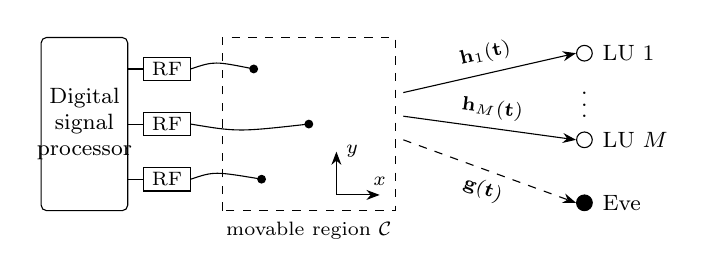
\begin{tikzpicture}[font=\footnotesize,>=Stealth]
  % BS baseband and RF chains
  \draw[rounded corners=2pt] (0,0.1) rectangle (1.1,2.3);
  \node[align=center] at (0.55,1.2) {Digital\\signal\\processor};
  \foreach \y in {1.9,1.2,0.5}{
    \draw (1.3,\y-0.15) rectangle (1.9,\y+0.15);
    \node at (1.6,\y) {\scriptsize RF};
    \draw (1.1,\y) -- (1.3,\y);}
  % movable region
  \draw[dashed] (2.3,0.1) rectangle (4.5,2.3);
  \node at (3.4,-0.15) {\scriptsize movable region $\mathcal C$};
  \foreach \x/\y in {2.7/1.9, 3.4/1.2, 2.8/0.5}{\fill (\x,\y) circle (1.6pt);}
  \draw (1.9,1.9) .. controls (2.2,2.0) .. (2.7,1.9);
  \draw (1.9,1.2) .. controls (2.5,1.1) .. (3.4,1.2);
  \draw (1.9,0.5) .. controls (2.2,0.6) .. (2.8,0.5);
  \draw[->] (3.75,0.3) -- (4.3,0.3) node[above] {\scriptsize $x$};
  \draw[->] (3.75,0.3) -- (3.75,0.85) node[right] {\scriptsize $y$};
  % receivers
  \node[draw,circle,inner sep=2pt] (u1) at (6.9,2.1) {};
  \node[anchor=west] at (u1.east) {LU $1$};
  \node at (6.9,1.55) {$\vdots$};
  \node[draw,circle,inner sep=2pt] (uM) at (6.9,1.0) {};
  \node[anchor=west] at (uM.east) {LU $M$};
  \node[draw,circle,fill=black,inner sep=2pt] (ev) at (6.9,0.2) {};
  \node[anchor=west] at (ev.east) {Eve};
  \draw[->] (4.6,1.6) -- (u1.west) node[midway,above,sloped] {\scriptsize $\mathbf h_1(\mathbf t)$};
  \draw[->] (4.6,1.3) -- (uM.west) node[midway,above,sloped] {\scriptsize $\mathbf h_M(\mathbf t)$};
  \draw[->,dashed] (4.6,1.0) -- (ev.west) node[midway,below,sloped] {\scriptsize $\mathbf g(\mathbf t)$};
\end{tikzpicture}
\caption{An MA-enabled multiuser downlink system in the presence of a passive eavesdropper.}
\label{fig:system}
\end{figure}

As shown in Fig.~\ref{fig:system}, we consider the downlink of a multiuser system, where a base station (BS) equipped with $N$ MAs serves $M$ single-antenna LUs in the presence of a single-antenna passive Eve. The LUs and the MAs are indexed by $m\in\mathcal M\triangleq\{1,\ldots,M\}$ and $n\in\mathcal N\triangleq\{1,\ldots,N\}$, respectively, where $N\ge M+1$ so that AN can be transmitted in the null space of the LU channels. The MAs are connected to the RF chains via flexible cables and can move within a two-dimensional (2D) square region $\mathcal C\triangleq[-A/2,A/2]\times[-A/2,A/2]$~\cite{ZhuMag2024,ZhuTWC2024Model}. The position of the $n$-th MA is $\bt_n\triangleq[x_n,y_n]^T\in\mathcal C$, and $\bt\triangleq[\bt_1^T,\ldots,\bt_N^T]^T$. To avoid the coupling between adjacent antennas, $\|\bt_n-\bt_i\|\ge\Dmin$, $\forall n\neq i$.

Since the size of $\mathcal C$ is much smaller than the propagation distance, moving the MAs changes only the phase of the LoS path, whereas its angle of departure (AoD) and amplitude remain unchanged~\cite{ZhuTWC2024Model}. Let $\theta_m\in[-\pi/2,\pi/2]$ and $\phi_m\in[-\pi/2,\pi/2]$ denote the elevation and azimuth AoDs of the LoS path from the BS to LU~$m$, respectively, and $\ba_m\triangleq[\cos\theta_m\sin\phi_m,\ \sin\theta_m]^T$. Then, the LoS component of the channel from the BS to LU $m$ is given by~\cite{ZhengTCOM2025}
\begin{equation}\label{eq:hbar}
\hb_m(\bt)\triangleq\Big[e^{j\frac{2\pi}{\lambda}\bt_1^T\ba_m},\ldots,e^{j\frac{2\pi}{\lambda}\bt_N^T\ba_m}\Big]^T\in\mathbb C^{N\times1},
\end{equation}
where $\lambda$ is the carrier wavelength. Following~\cite{ZhengTCOM2025,HuTVT2025}, the channel from the BS to LU $m$ is modeled as Rician fading, i.e.,
\begin{equation}\label{eq:hm}
\bh_m(\bt)=\sqrt{\frac{\kappa_m\beta_m}{\kappa_m+1}}\,\hb_m(\bt)+\sqrt{\frac{\beta_m}{\kappa_m+1}}\,\htl_m,
\end{equation}
where $\beta_m$ is the large-scale fading coefficient, $\kappa_m\ge0$ is the Rician factor, and $\htl_m\sim\CN(\mathbf 0,\bI_N)$ is the NLoS component.\footnote{As in~\cite{ZhengTCOM2025,HuTVT2025}, the NLoS components at different antennas are assumed to be independent and identically distributed (i.i.d.), which is reasonable in rich-scattering environments with $\Dmin\ge\lambda/2$.} Similarly, the channel from the BS to Eve is given by
\begin{equation}\label{eq:g}
\bg(\bt)=\sqrt{\frac{\kappa_e\beta_e}{\kappa_e+1}}\,\gb(\bt)+\sqrt{\frac{\beta_e}{\kappa_e+1}}\,\gtl,
\end{equation}
where $\beta_e$, $\kappa_e$, and $\gtl\sim\CN(\mathbf 0,\bI_N)$ are defined similarly to those in~\eqref{eq:hm}, and $\gb(\bt)$ is given by~\eqref{eq:hbar} with $\ba_m$ replaced by $\ba_e\triangleq[\cos\theta_e\sin\phi_e,\ \sin\theta_e]^T$, with $\theta_e$ and $\phi_e$ being the AoDs of Eve. The NLoS components $\htl_1,\ldots,\htl_M$ and $\gtl$ are mutually independent. We define $\bH(\bt)\triangleq[\bh_1(\bt),\ldots,\bh_M(\bt)]\in\mathbb C^{N\times M}$, $\Hb(\bt)\triangleq[\hb_1(\bt),\ldots,\hb_M(\bt)]$, $\Htl\triangleq[\htl_1,\ldots,\htl_M]$, and $\bK\triangleq\diag(\kappa_1,\ldots,\kappa_M)$. Note that the antenna positions affect the channels only through the LoS components $\Hb(\bt)$ and $\gb(\bt)$.

\subsection{Two-Timescale Transmission Protocol}

\begin{figure}[t]
\centering
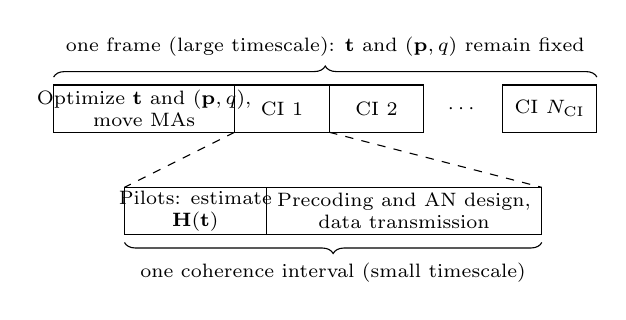
\begin{tikzpicture}[font=\scriptsize]
  \draw (0,0) rectangle (2.3,0.6);
  \node[align=center] at (1.15,0.3) {Optimize $\mathbf t$ and $(\mathbf p,q)$,\\move MAs};
  \draw (2.3,0) rectangle (3.5,0.6); \node at (2.9,0.3) {CI $1$};
  \draw (3.5,0) rectangle (4.7,0.6); \node at (4.1,0.3) {CI $2$};
  \node at (5.2,0.3) {$\cdots$};
  \draw (5.7,0) rectangle (6.9,0.6); \node at (6.3,0.3) {CI $N_{\mathrm{CI}}$};
  \draw[decorate,decoration={brace,amplitude=4pt}] (0,0.7) -- (6.9,0.7)
     node[midway,above=4pt] {one frame (large timescale): $\mathbf t$ and $(\mathbf p,q)$ remain fixed};
  \draw[dashed] (2.3,0) -- (0.9,-0.7);
  \draw[dashed] (3.5,0) -- (6.2,-0.7);
  \draw (0.9,-1.3) rectangle (2.7,-0.7);
  \node[align=center] at (1.8,-1.0) {Pilots: estimate\\$\mathbf H(\mathbf t)$};
  \draw (2.7,-1.3) rectangle (6.2,-0.7);
  \node[align=center] at (4.45,-1.0) {Precoding and AN design,\\data transmission};
  \draw[decorate,decoration={brace,mirror,amplitude=4pt}] (0.9,-1.4) -- (6.2,-1.4)
     node[midway,below=4pt] {one coherence interval (small timescale)};
\end{tikzpicture}
\caption{Illustration of the two-timescale transmission protocol (CI: coherence interval).}
\label{fig:protocol}
\end{figure}

Different from the instantaneous CSI over the entire region $\mathcal C$, whose acquisition requires the MAs to traverse the region~\cite{ZhengTCOM2025,HuTVT2025}, the statistical CSI, i.e., $\{\beta_m,\kappa_m,\theta_m,\phi_m\}_{m\in\mathcal M}$ of the LUs and $\{\beta_e,\kappa_e,\theta_e,\phi_e\}$ of Eve, is determined by the large-scale fading and the LoS geometry, which vary much more slowly than the small-scale fading. Following~\cite{HuTMC2024,ChenArxiv2026}, we assume that the statistical CSI of Eve is known at the BS, which can be obtained, e.g., from the prior knowledge of the location of Eve, by sensing its direction~\cite{ChenArxiv2026}, or from its historical signals if it is an untrusted node; the impact of errors in the AoD of Eve is evaluated in Section~\ref{sec:sim}.

Accordingly, we adopt the two-timescale protocol in Fig.~\ref{fig:protocol}. The time is divided into frames, each of which consists of $N_{\mathrm{CI}}\gg1$ CIs over which the statistical CSI remains constant. At the beginning of each frame, the BS optimizes the antenna positions $\bt$ and the long-term transmission parameters based on the statistical CSI, and moves the MAs accordingly. Then, in each CI, the BS estimates $\bH(\bt)$ via uplink pilots by exploiting the channel reciprocity of time-division duplexing, and designs the precoding and AN. For the purpose of exposition, $\bH(\bt)$ is assumed to be perfectly estimated, whereas $\gtl$ is never available at the BS. Compared with the instantaneous-CSI-based designs, the MAs are moved only once per frame, and the CSI of the LUs is required only at the current antenna positions.

\subsection{Signal Model}

In each CI, the BS transmits the confidential symbols $s_m\sim\CN(0,1)$, $m\in\mathcal M$, together with AN, i.e.,
\begin{equation}\label{eq:x}
\bx=\sum_{m=1}^{M}\bw_m s_m+\bz,
\end{equation}
where $\bw_m\in\mathbb C^{N\times1}$ is the precoding vector for LU $m$, and $\bz\sim\CN(\mathbf 0,\bSig)$ is the AN, which is independent of the mutually independent symbols $\{s_m\}$. Under the two-timescale protocol, $\{\bw_m\}$ and $\bSig$ are functions of the instantaneous CSI of the LUs, which are denoted by $\bw_m(\bH)$ and $\bSig(\bH)$ when necessary, and the transmit power is limited by $\sum_{m=1}^M\|\bw_m\|^2+\tr(\bSig)\le\Ptot$.

The signal received at LU $m$ is $y_m=\bh_m^H(\bt)\bx+n_m$ with $n_m\sim\CN(0,\sigma_m^2)$, and its signal-to-interference-plus-noise ratio (SINR) is
\begin{equation}\label{eq:sinr_gen}
\gamma_m=\frac{|\bh_m^H\bw_m|^2}{\sum_{i\in\mathcal M\setminus\{m\}}|\bh_m^H\bw_i|^2+\bh_m^H\bSig\bh_m+\sigma_m^2},
\end{equation}
where the dependence of the channels on $\bt$ is omitted for brevity. The signal received at Eve is $y_e=\bg^H(\bt)\bx+n_e$ with $n_e\sim\CN(0,\sigma_e^2)$. Since the receiver of a passive Eve is unknown to the BS, we consider the worst case where Eve can cancel the signals of the other LUs when intercepting $s_m$, e.g., via multiuser detection~\cite{ZhuTWC2014}, which yields a secrecy guarantee regardless of the decoding capability of Eve. The SINR of Eve for $s_m$ is then
\begin{equation}\label{eq:sinre_gen}
\gamma_{e,m}=\frac{|\bg^H\bw_m|^2}{\bg^H\bSig\bg+\sigma_e^2},
\end{equation}
which upper-bounds that of an Eve treating the signals of the other LUs as interference. The latter case is also evaluated in Section~\ref{sec:sim}.

\subsection{Ergodic Secrecy Rate and Problem Formulation}

Since the instantaneous CSI of Eve is unknown, the confidential message of each LU is encoded over the CIs of a frame, which experience independent realizations of the NLoS components. By coding over these fading realizations, the following ergodic secrecy rate is achievable for LU $m$~\cite{Gopala2008,ZhuTWC2014}:
\begin{equation}\label{eq:esr}
R_m^{\mathrm{sec}}\triangleq\big[\bar R_m-\bar R_{e,m}\big]^+,
\end{equation}
where
\begin{equation}\label{eq:ergodic}
\bar R_m\triangleq\E\{\log_2(1+\gamma_m)\},\quad \bar R_{e,m}\triangleq\E\{\log_2(1+\gamma_{e,m})\}
\end{equation}
denote the ergodic rate of LU $m$ and the ergodic wiretap rate of Eve for $s_m$, respectively, and the expectations are taken over $\Htl$ and $\gtl$ for given $\bt$. We aim to maximize the ESSR by jointly optimizing the long-term antenna positions and the short-term precoding and AN design policies, i.e.,
\begin{subequations}\label{eq:P1}
\begin{align}
(\mathrm{P1}):\ \max_{\bt,\{\bw_m(\cdot)\},\bSig(\cdot)}\ \ & \sum_{m=1}^{M}R_m^{\mathrm{sec}}\label{eq:P1obj}\\
\mathrm{s.t.}\ \ & \sum_{m=1}^M\|\bw_m(\bH)\|^2+\tr\big(\bSig(\bH)\big)\le\Ptot,\nonumber\\
& \bSig(\bH)\succeq\mathbf 0,\ \forall\bH,\label{eq:P1pow}\\
& \bt_n\in\mathcal C,\ \forall n\in\mathcal N,\label{eq:P1region}\\
& \|\bt_n-\bt_i\|\ge\Dmin,\ \forall n\neq i.\label{eq:P1dist}
\end{align}
\end{subequations}
Problem (P1) is challenging since the short-timescale variables are policies, i.e., mappings from the instantaneous CSI of the LUs to the precoders and the AN covariance matrix, which cannot be optimized in each CI separately because $\bar R_{e,m}$ is averaged over all CIs; the ergodic rates in~\eqref{eq:ergodic} have no closed-form expressions; and $\bt$ is coupled with the policies, while~\eqref{eq:P1dist} is non-convex. Stochastic optimization based on channel samples~\cite{ZhaoTWC2021} can be applied, but its complexity increases with the number of samples, and it provides little insight into the role of the MAs. Hence, we restrict the short-timescale design to ZF precoding and null-space AN with a long-term power allocation, which leads to tractable ergodic rates.

% =============================================================================
\section{Two-Timescale ZF-AN Design and Ergodic Secrecy Rate Analysis}\label{sec:analysis}
% =============================================================================

\subsection{Short-Timescale ZF Precoding and Null-Space AN}\label{sec:zfan}

Given $\bt$ and $\bH=\bH(\bt)$ in a CI, the BS adopts ZF precoding with a long-term power allocation, i.e., $\bw_m=\sqrt{p_m}\,\wb_m$, where $p_m\ge0$ is the power allocated to LU $m$, and
\begin{equation}\label{eq:zf}
\wb_m\triangleq\frac{\bH(\bH^H\bH)^{-1}\be_m}{\big\|\bH(\bH^H\bH)^{-1}\be_m\big\|}
\end{equation}
is the normalized ZF precoding direction of LU $m$, which satisfies $\bh_i^H\wb_m=0$, $\forall i\neq m$. Meanwhile, the AN is isotropically distributed in the null space of $\bH^H$~\cite{Zhou2010,ZhuTWC2014}, i.e.,
\begin{equation}\label{eq:an}
\bSig=q\,\PHp,\qquad \PHp\triangleq\bI_N-\bH(\bH^H\bH)^{-1}\bH^H,
\end{equation}
where $q\ge0$ denotes the AN power per dimension. Since $\PHp$ is the orthogonal projection onto the null space of $\bH^H$, whose dimension is $N-M$ with probability one, we have $\bH^H\PHp=\mathbf 0$ and $\tr(\PHp)=N-M$. Hence, the AN causes no interference to the LUs, and the transmit power in each CI is $\sum_{m=1}^M p_m+(N-M)q$. The power allocation $(\bp,q)$, where $\bp\triangleq[p_1,\ldots,p_M]^T$, is optimized based on the statistical CSI and remains fixed within a frame, whereas $\{\wb_m\}$ and $\PHp$ are updated in each CI. With this design, the SINRs in~\eqref{eq:sinr_gen} and~\eqref{eq:sinre_gen} reduce to
\begin{align}
\gamma_m&=\frac{p_m|\bh_m^H\wb_m|^2}{\sigma_m^2}=\frac{p_m}{\sigma_m^2\big[(\bH^H\bH)^{-1}\big]_{m,m}},\label{eq:snr}\\
\gamma_{e,m}&=\frac{p_m|\bg^H\wb_m|^2}{q\,\bg^H\PHp\bg+\sigma_e^2},\label{eq:sinre}
\end{align}
respectively, where the second equality in~\eqref{eq:snr} holds since $\bh_m^H\bH(\bH^H\bH)^{-1}\be_m=1$ and $\|\bH(\bH^H\bH)^{-1}\be_m\|^2=[(\bH^H\bH)^{-1}]_{m,m}$.

The adopted ZF-AN design requires only the instantaneous CSI of the LUs, eliminates both the inter-user interference and the AN at the LUs, and solves no optimization problem in each CI, since $(\bp,q)$ is adapted only to the statistical CSI. The equal power allocation in~\cite{ZhengTCOM2025} and the information--AN power splitting with equal power among the LUs are special cases of this power allocation. With the ZF-AN design, (P1) is transformed into
\begin{subequations}\label{eq:P2}
\begin{align}
(\mathrm{P2}):\ \max_{\bt,\bp,q}\ \ & \sum_{m=1}^{M}R_m^{\mathrm{sec}}(\bt,p_m,q)\label{eq:P2obj}\\
\mathrm{s.t.}\ \ & \sum_{m=1}^{M}p_m+(N-M)q\le\Ptot,\label{eq:P2pow}\\
& p_m\ge0,\ \forall m\in\mathcal M,\quad q\ge0,\label{eq:P2pos}\\
& \eqref{eq:P1region},\ \eqref{eq:P1dist},\nonumber
\end{align}
\end{subequations}
where $R_m^{\mathrm{sec}}(\bt,p_m,q)$ denotes~\eqref{eq:esr} with the SINRs in~\eqref{eq:snr} and~\eqref{eq:sinre}. Since the ergodic rates still have no closed-form expressions, we derive their approximations in the sequel.

\subsection{Ergodic Rate of the LUs}\label{sec:lu}

Define $\bB\triangleq\diag\big(\frac{\beta_1}{\kappa_1+1},\ldots,\frac{\beta_M}{\kappa_M+1}\big)$ and $\bL(\bt)\triangleq\Hb(\bt)\bK^{1/2}$. From~\eqref{eq:hm}, the channel matrix of the LUs can be written as
\begin{equation}\label{eq:Hdecomp}
\bH(\bt)=\big(\bL(\bt)+\Htl\big)\bB^{1/2},
\end{equation}
where $\bL(\bt)+\Htl$ is the normalized channel matrix, whose LoS component is weighted by the square roots of the Rician factors. Accordingly, we define
\begin{equation}\label{eq:Phi}
\bPhi(\bt)\triangleq\bL^H(\bt)\bL(\bt)+N\bI_M,\qquad \bOm(\bt)\triangleq\bPhi^{-1}(\bt),
\end{equation}
where $\bPhi(\bt)=\E\{(\bL(\bt)+\Htl)^H(\bL(\bt)+\Htl)\}$ is the correlation matrix of the normalized channels of the LUs.

\begin{lemma}\label{lem:lu}
For given $\bt$ and $p_m$, the ergodic rate of LU $m$ is approximated by~\cite{ZhangJSTSP2014,ZhengTCOM2025}
\begin{equation}\label{eq:Rm}
\bar R_m\approx\tilde R_m(\bt,p_m)\triangleq\log_2\big(1+\eta_m(\bt)\,p_m\big),
\end{equation}
where $\eta_m(\bt)\triangleq\zeta_m(N-M)/(N\omega_m(\bt))$, $\zeta_m\triangleq\beta_m/((\kappa_m+1)\sigma_m^2)$, and $\omega_m(\bt)\triangleq[\bOm(\bt)]_{m,m}$.
\end{lemma}
\begin{IEEEproof}
By applying Jensen's inequality to the convex function $\log_2(1+1/x)$ of $x>0$, we have $\bar R_m\ge\log_2\big(1+p_m/(\sigma_m^2\E\{[(\bH^H\bH)^{-1}]_{m,m}\})\big)$. Following~\cite{ZhangJSTSP2014}, the noncentral Wishart matrix $(\bL+\Htl)^H(\bL+\Htl)$ is approximated by a central Wishart matrix with $N$ degrees of freedom and the same mean $\bPhi(\bt)$, whose inverse has the mean $N\bOm(\bt)/(N-M)$. Together with~\eqref{eq:Hdecomp}, this yields $\E\{[(\bH^H\bH)^{-1}]_{m,m}\}\approx N(\kappa_m+1)\omega_m(\bt)/(\beta_m(N-M))$, which leads to~\eqref{eq:Rm}.
\end{IEEEproof}

Lemma~\ref{lem:lu} is equivalent to the approximation in~\cite[Sec.~IV-A]{ZhengTCOM2025}, since the normalized channel correlation matrix used therein equals $\frac1N(\bK+\bI_M)^{-1/2}\bPhi(\bt)(\bK+\bI_M)^{-1/2}$. Since $\bPhi(\bt)\succeq N\bI_M$ and $[\bOm(\bt)]_{m,m}\ge1/[\bPhi(\bt)]_{m,m}=1/(N(\kappa_m+1))$~\cite{Horn2013}, we have
\begin{equation}\label{eq:etabound}
\zeta_m(N-M)\le\eta_m(\bt)\le\zeta_m(N-M)(\kappa_m+1),
\end{equation}
where the upper bound is achieved if $\hb_m^H(\bt)\hb_i(\bt)=0$ for all $i\neq m$ with $\kappa_i>0$. Hence, $1/(N\omega_m(\bt))\in[1,\kappa_m+1]$ is the LoS gain of LU $m$ that survives the ZF precoding, which can be improved by decorrelating the LoS components of the LUs via the antenna positions.

\remarkhead{Accuracy of Lemma~\ref{lem:lu}}\label{rem:lu} Lemma~\ref{lem:lu} is a lower-bound-type approximation, which is exact for Rayleigh fading, i.e., $\bK=\mathbf 0$, where~\eqref{eq:Rm} reduces to the well-known lower bound $\log_2(1+\zeta_mp_m(N-M))$~\cite{Ngo2013}. For large Rician factors, the degrees-of-freedom loss $(N-M)/N$ also applies to the deterministic LoS component, and the gap between~\eqref{eq:Rm} and $\bar R_m$ approaches $\log_2(N/(N-M))$ at high SNR as $\kappa_i\to\infty$, $\forall i\in\mathcal M$. Since this gap depends mainly on the Rician factors and $N/(N-M)$, and only weakly on $\bt$ (see Section~\ref{sec:sim}), we adopt~\eqref{eq:Rm} due to its simplicity~\cite{ZhengTCOM2025,HuTVT2025} and focus on the ergodic wiretap rate of Eve, for which no existing result is available.

\subsection{Ergodic Wiretap Rate of Eve}\label{sec:eve}

The SINR of Eve in~\eqref{eq:sinre} depends on the random ZF direction and AN subspace induced by $\bH$. The following lemma characterizes the information leakage and the AN received by Eve conditioned on $\bH$.

\begin{lemma}\label{lem:indep}
Conditioned on $\bH$, the information leakage $X_m\triangleq|\bg^H\wb_m|^2$ and the AN power $Y\triangleq\bg^H\PHp\bg$ received by Eve are independent, and their conditional means and variances are given by
\begin{align}
\E\{X_m|\bH\}&=\tilde\beta_e\big(\kappa_ex_m+1\big),\nonumber\\
\mathrm{Var}\{X_m|\bH\}&=\tilde\beta_e^2\big(2\kappa_ex_m+1\big),\label{eq:EX}\\
\E\{Y|\bH\}&=\tilde\beta_e\big(\kappa_ey+N-M\big),\nonumber\\
\mathrm{Var}\{Y|\bH\}&=\tilde\beta_e^2\big(2\kappa_ey+N-M\big),\label{eq:EY}
\end{align}
where $\tilde\beta_e\triangleq\beta_e/(\kappa_e+1)$, $x_m\triangleq|\gb^H\wb_m|^2$, and $y\triangleq\gb^H\PHp\gb$.
\end{lemma}
\begin{IEEEproof}
Let $\mathbf U\triangleq[\mathbf u_1,\ldots,\mathbf u_{N-M}]$ be an orthonormal basis of the null space of $\bH^H$, so that $\PHp=\mathbf U\mathbf U^H$ and $Y=\sum_{i=1}^{N-M}|\mathbf u_i^H\bg|^2$. Since $\wb_m$ is a unit-norm vector in the column space of $\bH$, the matrix $[\wb_m,\mathbf U]$ has orthonormal columns. Since $\gtl$ is independent of $\bH$, we have $\bg|\bH\sim\CN(\sqrt{\kappa_e\tilde\beta_e}\,\gb,\tilde\beta_e\bI_N)$ from~\eqref{eq:g}, and thus $\wb_m^H\bg,\mathbf u_1^H\bg,\ldots,\mathbf u_{N-M}^H\bg$ are independent complex Gaussian random variables with variance $\tilde\beta_e$ given $\bH$. Hence, $X_m=|\wb_m^H\bg|^2$ and $Y$ are conditionally independent. Finally, \eqref{eq:EX} and~\eqref{eq:EY} follow from $\E\{|z|^2\}=|\mu|^2+\sigma^2$ and $\mathrm{Var}\{|z|^2\}=\sigma^4+2|\mu|^2\sigma^2$ for $z\sim\CN(\mu,\sigma^2)$, together with $\sum_{i=1}^{N-M}|\mathbf u_i^H\gb|^2=y$.
\end{IEEEproof}

Lemma~\ref{lem:indep} shows that, given the channels of the LUs, the information leakage is determined only by the component of the wiretap channel along the ZF direction, whereas the AN received by Eve is determined only by its component in the null space of $\bH^H$. Moreover, the conditional relative variances of $X_m$ and $Y$ are $(2\kappa_ex_m+1)/(\kappa_ex_m+1)^2$ and $(2\kappa_ey+N-M)/(\kappa_ey+N-M)^2$, i.e., $X_m$ concentrates when the LoS leakage $\kappa_ex_m$ is strong, which dominates the ergodic wiretap rate, and $Y$ concentrates when $N-M$ or $\kappa_ey$ is large. This motivates the approximation $\E\{\log_2(1+X/Y)\}\approx\log_2(1+\E\{X\}/\E\{Y\})$~\cite[Lemma~1]{ZhangJSTSP2014}, which is accurate when $X$ and $Y$ concentrate around their means and asymptotically exact as $\kappa_e,\kappa_m\to\infty$, $\forall m$. Using Lemma~\ref{lem:indep} and taking the expectation over $\Htl$, we obtain
\begin{equation}\label{eq:Re0}
\bar R_{e,m}\approx\log_2\bigg(1+\frac{p_m\big(\kappa_e\E\{x_m\}+1\big)}{q\big(\kappa_e\E\{y\}+N-M\big)+\sbe}\bigg),
\end{equation}
where $\sbe\triangleq\sigma_e^2/\tilde\beta_e=\sigma_e^2(\kappa_e+1)/\beta_e$ is the normalized noise power of Eve.

The expectations $\E\{x_m\}=\E\{|\gb^H\wb_m|^2\}$ and $\E\{y\}=\E\{\gb^H\PHp\gb\}$ in~\eqref{eq:Re0} are the average LoS energies of Eve along the ZF direction of LU $m$ and in the AN subspace, respectively, which have no closed-form expressions. Since $\wb_m$ and $\PHp$ are invariant to the scaling of the columns of $\bH$, they can be computed based on the normalized channel matrix $\bL(\bt)+\Htl$ in~\eqref{eq:Hdecomp}, which motivates the following lemma for a generic noncentral Gaussian matrix.

\begin{lemma}\label{lem:det}
Let $\bF=\Fb+\bW\in\mathbb C^{N\times k}$ with $k<N$, where $\Fb$ is deterministic and the entries of $\bW$ are i.i.d. $\CN(0,1)$ random variables. Let $\bb\in\mathbb C^{N\times1}$ be a deterministic vector, and define $\bPhi_{\bF}\triangleq\E\{\bF^H\bF\}=\Fb^H\Fb+N\bI_k$, $\wb_m(\bF)\triangleq\bF(\bF^H\bF)^{-1}\be_m/\|\bF(\bF^H\bF)^{-1}\be_m\|$, and $\mathbf P_{\bF}^\perp\triangleq\bI_N-\bF(\bF^H\bF)^{-1}\bF^H$. Then, we have
\begin{align}
\E\{|\bb^H\wb_m(\bF)|^2\}&\approx\frac{\big|[\bPhi_{\bF}^{-1}\Fb^H\bb]_m\big|^2+\|\bb\|^2[\bPhi_{\bF}^{-2}]_{m,m}}{[\bPhi_{\bF}^{-1}]_{m,m}},\label{eq:lem_c}\\
\E\{\bb^H\mathbf P_{\bF}^\perp\bb\}&\approx\frac{(N-k)\big(\|\bb\|^2-\bb^H\Fb\bPhi_{\bF}^{-1}\Fb^H\bb\big)}{N-k+N\tr(\bPhi_{\bF}^{-1})}.\label{eq:lem_d}
\end{align}
Moreover, \eqref{eq:lem_c} and~\eqref{eq:lem_d} are exact for $\Fb=\mathbf 0$, and are asymptotically exact for $\Fb=\varrho\Fb_0$ as $\varrho\to\infty$, where $\Fb_0$ has full column rank. The right-hand sides of~\eqref{eq:lem_c} and~\eqref{eq:lem_d} lie in $[0,\|\bb\|^2]$, as do their left-hand sides.
\end{lemma}
\begin{IEEEproof}
See Appendix~\ref{app:det}.
\end{IEEEproof}

Lemma~\ref{lem:det} replaces the random matrix $(\bF^H\bF)^{-1}$ by the inverse of its mean, which is accurate when the LoS component dominates or $N$ is large compared with $k$. In~\eqref{eq:lem_d}, the NLoS component is further restricted to the part of the space that is not captured by the LoS component, and its share is calibrated by the identity $\tr(\mathbf P_{\bF}^\perp)=N-k$, which holds for every realization of $\bF$ (see Appendix~\ref{app:det}). Applying Lemma~\ref{lem:det} to~\eqref{eq:Re0} yields the following closed-form approximation.

\begin{proposition}\label{prop:eve}
Define $\bv(\bt)\triangleq\bL^H(\bt)\gb(\bt)=\bK^{1/2}\Hb^H(\bt)\gb(\bt)$ and
\begin{align}
c_m(\bt)&\triangleq\frac{\big|[\bOm(\bt)\bv(\bt)]_m\big|^2+N[\bOm^2(\bt)]_{m,m}}{\omega_m(\bt)},\label{eq:cm}\\
d(\bt)&\triangleq\frac{(N-M)\big(N-\bv^H(\bt)\bOm(\bt)\bv(\bt)\big)}{N-M+N\tr(\bOm(\bt))}.\label{eq:d}
\end{align}
Then, the ergodic wiretap rate of Eve for $s_m$ is approximated by
\begin{equation}\label{eq:Re}
\bar R_{e,m}\approx\tilde R_{e,m}(\bt,p_m,q)\triangleq\log_2\bigg(1+\frac{\xi_m(\bt)\,p_m}{q\,\psi(\bt)+\sbe}\bigg),
\end{equation}
where $\xi_m(\bt)\triangleq\kappa_ec_m(\bt)+1$ and $\psi(\bt)\triangleq\kappa_ed(\bt)+N-M$.
\end{proposition}
\begin{IEEEproof}
From~\eqref{eq:Hdecomp}, $\wb_m=\wb_m(\bL(\bt)+\Htl)$ and $\PHp=\mathbf P_{\bL(\bt)+\Htl}^\perp$. Applying Lemma~\ref{lem:det} with $\Fb=\bL(\bt)$, $\bW=\Htl$, $k=M$, and $\bb=\gb(\bt)$, for which $\bPhi_{\bF}=\bPhi(\bt)$, $\Fb^H\bb=\bv(\bt)$, and $\|\bb\|^2=N$, yields $\E\{x_m\}\approx c_m(\bt)$ and $\E\{y\}\approx d(\bt)$. Substituting them into~\eqref{eq:Re0} completes the proof.
\end{IEEEproof}

In Proposition~\ref{prop:eve}, $c_m(\bt)\in[0,N]$ and $d(\bt)\in[0,N]$ approximate the LoS energy of Eve along the ZF direction of LU $m$ and in the AN subspace, respectively, so that $\xi_m(\bt)$ and $\psi(\bt)$ are the normalized information leakage for LU $m$ and the normalized AN power received by Eve. Different from the existing approximations for ZF precoding, which only involve the diagonal entries of $\bOm(\bt)$, Proposition~\ref{prop:eve} captures the correlation between the LoS components of Eve and the LUs via $\bv(\bt)$.

\subsection{Approximate ESSR and Discussions}\label{sec:discussion}

Based on Lemma~\ref{lem:lu} and Proposition~\ref{prop:eve}, the ergodic secrecy rate of LU $m$ is approximated by
\begin{equation}\label{eq:esrapprox}
R_m^{\mathrm{sec}}\approx\tilde R_m^{\mathrm{sec}}(\bt,p_m,q)\triangleq\big[\tilde R_m(\bt,p_m)-\tilde R_{e,m}(\bt,p_m,q)\big]^+,
\end{equation}
which depends only on the statistical CSI and is thus suitable for the large-timescale design. The insights revealed by~\eqref{eq:esrapprox} are discussed below.

\remarkhead{Role of the antenna positions}\label{rem:role} From~\eqref{eq:Rm}, \eqref{eq:cm}, and~\eqref{eq:d}, the antenna positions affect the approximate ESSR only through three geometric quantities, i.e., $\omega_m(\bt)$, $c_m(\bt)$, and $d(\bt)$, which depend on $\bt$ only via $\bPhi(\bt)$ and $\bv(\bt)$, i.e., via the LoS array correlations $[\Hb^H(\bt)\Hb(\bt)]_{i,j}=\sum_{n=1}^{N}e^{j\frac{2\pi}{\lambda}\bt_n^T(\ba_j-\ba_i)}$ among the LUs and $[\Hb^H(\bt)\gb(\bt)]_{i}=\sum_{n=1}^{N}e^{j\frac{2\pi}{\lambda}\bt_n^T(\ba_e-\ba_i)}$ between Eve and the LUs. A smaller $\omega_m(\bt)$ indicates that the LoS component of LU $m$ is less correlated with those of the other LUs, which yields a larger ZF gain; a smaller $c_m(\bt)$ indicates less information leakage; and a larger $d(\bt)$ indicates more AN received by Eve. In particular, if $\bv(\bt)=\mathbf 0$, i.e., the LoS component of Eve is orthogonal to those of all the LUs, then $c_m(\bt)$ reduces to its minimum $N[\bOm^2(\bt)]_{m,m}/\omega_m(\bt)$ caused by the NLoS components, and $d(\bt)$ achieves its maximum $N(N-M)/(N-M+N\tr(\bOm(\bt)))$ for a given $\bPhi(\bt)$. Hence, by decorrelating the LoS component of Eve from those of the LUs, the MAs simultaneously reduce the information leakage and increase the AN received by Eve, which is difficult for an FPA array when Eve is located in a direction close to that of an LU.

\remarkhead{Special cases}\label{rem:special} 1) If $\kappa_e=0$, then $\tilde R_{e,m}=\log_2(1+p_m/(q(N-M)+\sbe))$ does not depend on $\bt$, i.e., the statistical CSI of Eve carries no spatial information, and the MAs enhance secrecy only by improving $\omega_m(\bt)$ as in the rate-oriented design. 2) If $M=1$, then $\bPhi(\bt)=N(\kappa_1+1)$ is a scalar, and $\eta_1=\zeta_1(N-1)(\kappa_1+1)$ does not depend on $\bt$.\footnote{In fact, for $M=1$, the exact ergodic rate $\E\{\log_2(1+p_1\|\bh_1\|^2/\sigma_1^2)\}$ does not depend on $\bt$, since the distribution of $\|\bh_1\|^2$ depends on $\hb_1(\bt)$ only through $\|\hb_1(\bt)\|^2=N$.} In contrast,
\begin{align}
c_1(\bt)&=\frac{\kappa_1|\hb_1^H(\bt)\gb(\bt)|^2/N+1}{\kappa_1+1},\label{eq:c1}\\
d(\bt)&=\frac{(N-1)(\kappa_1+1)}{(N-1)(\kappa_1+1)+1}\bigg(N-\frac{\kappa_1|\hb_1^H(\bt)\gb(\bt)|^2}{N(\kappa_1+1)}\bigg)\label{eq:d1}
\end{align}
depend on $\bt$ through the LoS correlation $|\hb_1^H(\bt)\gb(\bt)|^2$ between the LU and Eve. Hence, different from the rate-oriented two-timescale design, where the MAs bring no gain for a single user~\cite{ZhengTCOM2025}, the MAs enhance the secrecy of a single LU by reducing this correlation.

\remarkhead{High-SNR behavior and AN saving}\label{rem:highsnr} Consider the information--AN power splitting with equal power among the LUs, i.e., $p_m=\alpha\Ptot/M$ and $q=(1-\alpha)\Ptot/(N-M)$ with $\alpha\in(0,1)$. As $\Ptot\to\infty$, we have
\begin{equation}\label{eq:highsnr}
\tilde R_m-\tilde R_{e,m}=\log_2\frac{\alpha\Ptot\eta_m(\bt)}{M}-\log_2\Big(1+\frac{\alpha\Theta_m(\bt)}{1-\alpha}\Big)+o(1),
\end{equation}
where $\Theta_m(\bt)\triangleq\frac{(N-M)\xi_m(\bt)}{M\psi(\bt)}$ is the ratio of the normalized information leakage to the normalized AN power received by Eve. Hence, the high-SNR slope of the ESSR equals $M$ regardless of $\bt$, and the antenna positions affect the ESSR through the constant term. Moreover, the value of $\alpha$ that maximizes the sum of the constant terms in~\eqref{eq:highsnr} is the root of $\sum_{m=1}^M\big[\frac1\alpha-\frac1{1-\alpha}-\frac{\Theta_m-1}{1+\alpha(\Theta_m-1)}\big]=0$, which, for $\Theta_m=\Theta$, $\forall m$, is given by
\begin{equation}\label{eq:alphastar}
\alpha^\star=\frac{1}{1+\sqrt{\Theta}}.
\end{equation}
Since the MAs can decrease $c_m(\bt)$ and increase $d(\bt)$, they decrease $\Theta$ and thus increase $\alpha^\star$, i.e., they reduce the AN power required for secure transmission, which is referred to as the AN-saving effect.

% =============================================================================
\section{Proposed Two-Timescale Optimization Algorithm}\label{sec:opt}
% =============================================================================

\subsection{Problem Reformulation}

By replacing the ergodic secrecy rates in (P2) with their approximations in~\eqref{eq:esrapprox}, we consider the following problem, which depends only on the statistical CSI:
\begin{subequations}\label{eq:P3}
\begin{align}
(\mathrm{P3}):\ \max_{\bt,\bp,q}\ \ & F(\bt,\bp,q)\triangleq\sum_{m=1}^{M}\bigg[\log_2\big(1+\eta_m(\bt)p_m\big)\nonumber\\
&\qquad\qquad-\log_2\bigg(1+\frac{\xi_m(\bt)p_m}{q\psi(\bt)+\sbe}\bigg)\bigg]\label{eq:P3obj}\\
\mathrm{s.t.}\ \ & \eqref{eq:P1region},\ \eqref{eq:P1dist},\ \eqref{eq:P2pow},\ \eqref{eq:P2pos},\nonumber
\end{align}
\end{subequations}
where the operator $[\cdot]^+$ in~\eqref{eq:esrapprox} is dropped without loss of optimality, as shown below.

\begin{proposition}\label{prop:plus}
The optimal value of (P3) equals that of the problem obtained by replacing $F(\bt,\bp,q)$ in~\eqref{eq:P3obj} with $\sum_{m=1}^M\tilde R_m^{\mathrm{sec}}(\bt,p_m,q)$. Moreover, at any optimal solution of (P3), every term in the summation of~\eqref{eq:P3obj} is nonnegative.
\end{proposition}
\begin{IEEEproof}
Since $[x]^+\ge x$, the optimal value with $[\cdot]^+$ is no smaller than that of (P3). Conversely, for any feasible $(\bt,\bp,q)$, let $\bp'$ be obtained by setting $p_m'=0$ for all $m$ with $\tilde R_m(\bt,p_m)<\tilde R_{e,m}(\bt,p_m,q)$ and $p_m'=p_m$ otherwise. Then, $(\bt,\bp',q)$ is feasible, and since the $m$-th term of $F$ depends only on $p_m$ and $q$ for a given $\bt$, we have $F(\bt,\bp',q)=\sum_{m=1}^M\tilde R_m^{\mathrm{sec}}(\bt,p_m,q)$. Hence, the two optimal values are equal. If some term were negative at an optimal solution of (P3), setting the corresponding $p_m$ to zero would strictly increase $F$, which is a contradiction.
\end{IEEEproof}

Proposition~\ref{prop:plus} shows that the non-smooth operator $[\cdot]^+$ can be removed by allowing the BS to switch off the LUs with non-positive secrecy rates, which is enabled by the per-user power allocation. In contrast, under equal power allocation among the LUs, the operator $[\cdot]^+$ must be retained. Since (P3) is still non-convex due to the coupling between $\bt$ and $(\bp,q)$ and the non-convex constraint~\eqref{eq:P1dist}, we adopt the AO framework, which alternately optimizes $(\bp,q)$ for given $\bt$ and $\bt$ for given $(\bp,q)$.

\subsection{Power Allocation Optimization}\label{sec:power}

For given $\bt$, the coefficients $\eta_m$, $\xi_m$, and $\psi$ are constants, and (P3) reduces to
\begin{equation}\label{eq:P31}
(\mathrm{P3.1}):\ \max_{\bp,q}\ \sum_{m=1}^{M}f_m(p_m;q)\quad\mathrm{s.t.}\ \eqref{eq:P2pow},\ \eqref{eq:P2pos},
\end{equation}
where
\begin{equation}\label{eq:fm}
f_m(p;q)\triangleq\log_2(1+\eta_mp)-\log_2\big(1+\eta_{e,m}(q)\,p\big),
\end{equation}
and $\eta_{e,m}(q)\triangleq\xi_m/(q\psi+\sbe)$ is the effective channel gain of Eve for LU $m$, which decreases with $q$. We first optimize $\bp$ for a given $q$. The first-order and second-order derivatives of $f_m$ with respect to (w.r.t.) $p$ are given by
\begin{align}
\frac{\partial f_m}{\partial p}&=\frac{\eta_m-\eta_{e,m}}{\ln2\,(1+\eta_mp)(1+\eta_{e,m}p)},\label{eq:fm1}\\
\frac{\partial^2 f_m}{\partial p^2}&=\frac{1}{\ln2}\bigg[\frac{\eta_{e,m}^2}{(1+\eta_{e,m}p)^2}-\frac{\eta_m^2}{(1+\eta_mp)^2}\bigg],\label{eq:fm2}
\end{align}
where the argument $q$ of $\eta_{e,m}$ is omitted. If $\eta_m\le\eta_{e,m}$, then $f_m(p;q)\le0$ for all $p\ge0$, and thus $p_m=0$ is optimal. If $\eta_m>\eta_{e,m}$, then $\eta_m(1+\eta_{e,m}p)-\eta_{e,m}(1+\eta_mp)=\eta_m-\eta_{e,m}>0$, i.e., $\frac{\eta_m}{1+\eta_mp}>\frac{\eta_{e,m}}{1+\eta_{e,m}p}$, which implies that $f_m$ is strictly increasing and strictly concave in $p\ge0$. Let $\mathcal M_{\mathrm a}(q)\triangleq\{m\in\mathcal M\,|\,\eta_m>\eta_{e,m}(q)\}$ denote the set of LUs that can achieve positive secrecy rates, and $P_{\mathrm I}(q)\triangleq\Ptot-(N-M)q$ the power available for the confidential signals. Then, for a given $q$, the optimization of $\bp$ is a convex problem, whose solution is given as follows.

\begin{proposition}[Secrecy water-filling]\label{prop:wf}
For a given $q$ with $P_{\mathrm I}(q)>0$ and $\mathcal M_{\mathrm a}(q)\neq\emptyset$, the optimal power allocation is $p_m^\star=0$ for $m\notin\mathcal M_{\mathrm a}(q)$ and
\begin{equation}\label{eq:wf}
p_m^\star(\nu)=\bigg[\frac{2(\rho_m-1)}{\sqrt{(\eta_m-\eta_{e,m})^2+4\eta_m\eta_{e,m}\rho_m}+\eta_m+\eta_{e,m}}\bigg]^+
\end{equation}
for $m\in\mathcal M_{\mathrm a}(q)$, where $\rho_m=\rho_m(\nu)\triangleq(\eta_m-\eta_{e,m})/(\nu\ln2)$, and the water level $\nu>0$ is the unique solution of $\sum_{m\in\mathcal M_{\mathrm a}(q)}p_m^\star(\nu)=P_{\mathrm I}(q)$.
\end{proposition}
\begin{IEEEproof}
Since the objective is strictly concave and increasing in $\{p_m\}_{m\in\mathcal M_{\mathrm a}(q)}$ and Slater's condition holds, the Karush--Kuhn--Tucker (KKT) conditions are necessary and sufficient for optimality, and the power constraint is active at the optimum~\cite{Boyd2004}. Let $\nu>0$ denote the dual variable associated with the power constraint. The KKT conditions yield $\partial f_m/\partial p=\nu$ if $p_m^\star>0$ and $\partial f_m/\partial p|_{p=0}\le\nu$ otherwise. From~\eqref{eq:fm1}, the former is equivalent to $(1+\eta_mp)(1+\eta_{e,m}p)=\rho_m(\nu)$, i.e., a quadratic equation in $p$, whose positive root, written in a numerically stable form, is given by~\eqref{eq:wf}. The latter is equivalent to $\rho_m(\nu)\le1$, in which case~\eqref{eq:wf} gives $p_m^\star=0$. Finally, since $\sum_{m\in\mathcal M_{\mathrm a}(q)}p_m^\star(\nu)$ is continuous and strictly decreasing in $\nu$ over $(0,\max_{m\in\mathcal M_{\mathrm a}(q)}(\eta_m-\eta_{e,m})/\ln2)$, ranging from $+\infty$ to $0$, the water level is unique.
\end{IEEEproof}

Note that~\eqref{eq:wf} reduces to the classic water-filling solution $[1/(\nu\ln2)-1/\eta_m]^+$ when $\eta_{e,m}\to0$. Hence, \eqref{eq:wf} can be regarded as a secrecy water-filling solution, in which the LUs whose effective channel gains do not exceed that of Eve are switched off. Since $p_m^\star(\nu)$ is non-increasing in $\nu$, the water level can be efficiently found by bisection.

Next, let $G(q)\triangleq\sum_{m\in\mathcal M}f_m(p_m^\star;q)$ denote the objective value achieved by the optimal $\bp$ for a given $q$, where $G(q)=0$ if $\mathcal M_{\mathrm a}(q)=\emptyset$ or $P_{\mathrm I}(q)=0$. The optimal AN power per dimension is obtained by solving
\begin{equation}\label{eq:qsearch}
q^\star=\arg\max_{0\le q\le q_{\max}}\ G(q),
\end{equation}
where $q_{\max}\triangleq\Ptot/(N-M)$. Increasing $q$ reduces the effective channel gains of Eve at the cost of less power for the confidential signals. Since $G(q)$ is not necessarily unimodal, \eqref{eq:qsearch} is solved by a coarse grid search followed by a fine grid search around the best grid point, as summarized in Algorithm~\ref{alg:power}.

\begin{algorithm}[t]
\caption{Power Allocation for Given $\bt$}\label{alg:power}
\begin{algorithmic}[1]
\Require $\{\eta_m,\xi_m\}_{m\in\mathcal M}$, $\psi$, $\Ptot$, and grid size $Q$.
\For{each $q$ in a uniform grid of $Q$ points over $[0,q_{\max}]$}
  \State Compute $\eta_{e,m}(q)$ and $\mathcal M_{\mathrm a}(q)$.
  \State Find $\nu$ by bisection such that $\sum_{m\in\mathcal M_{\mathrm a}(q)}p_m^\star(\nu)=P_{\mathrm I}(q)$, where $p_m^\star(\nu)$ is given by~\eqref{eq:wf}.
  \State Evaluate $G(q)$.
\EndFor
\State Repeat Steps 1--5 over a uniform grid of $Q$ points between the two neighbors of the best grid point.
\Ensure $q^\star$ and the corresponding $\bp^\star$.
\end{algorithmic}
\end{algorithm}

\subsection{Antenna Position Optimization}\label{sec:position}

For given $(\bp,q)$, (P3) reduces to
\begin{equation}\label{eq:P32}
(\mathrm{P3.2}):\ \max_{\bt}\ F(\bt)\quad\mathrm{s.t.}\ \eqref{eq:P1region},\ \eqref{eq:P1dist},
\end{equation}
where $F(\bt)\triangleq F(\bt,\bp,q)$, which is neither concave nor convex w.r.t. $\bt$. Similar to~\cite{ZhengTCOM2025}, we optimize the position of each MA in an element-wise manner with the other positions fixed, and update $\bt_n$ by the MM method~\cite{Sun2017}.

\textit{1) Dependence on $\bt_n$:} Let $\bl_n(\bt_n)\in\mathbb C^{M\times1}$ denote the conjugate transpose of the $n$-th row of $\bL(\bt)$, i.e.,
\begin{equation}\label{eq:ln}
\bl_n(\bt_n)=\bK^{1/2}\Big[e^{-j\frac{2\pi}{\lambda}\bt_n^T\ba_1},\ldots,e^{-j\frac{2\pi}{\lambda}\bt_n^T\ba_M}\Big]^T.
\end{equation}
Since $\bL^H\bL=\sum_{i=1}^N\bl_i\bl_i^H$ and $\bL^H\gb=\sum_{i=1}^N\bl_ie^{j\frac{2\pi}{\lambda}\bt_i^T\ba_e}$, we have
\begin{align}
\bPhi(\bt)&=\bGam_n+\bl_n(\bt_n)\bl_n^H(\bt_n),\label{eq:Phin}\\
\bv(\bt)&=\br_n+\bl_n(\bt_n)e^{j\frac{2\pi}{\lambda}\bt_n^T\ba_e},\label{eq:vn}
\end{align}
where $\bGam_n\triangleq\sum_{i\neq n}\bl_i(\bt_i)\bl_i^H(\bt_i)+N\bI_M$ and $\br_n\triangleq\sum_{i\neq n}\bl_i(\bt_i)e^{j\frac{2\pi}{\lambda}\bt_i^T\ba_e}$ do not depend on $\bt_n$. By the Sherman--Morrison formula~\cite{Horn2013},
\begin{equation}\label{eq:sm}
\bOm(\bt)=\bGam_n^{-1}-\frac{\bGam_n^{-1}\bl_n(\bt_n)\bl_n^H(\bt_n)\bGam_n^{-1}}{1+\bl_n^H(\bt_n)\bGam_n^{-1}\bl_n(\bt_n)}.
\end{equation}
Hence, for given $\bGam_n^{-1}$ and $\br_n$, evaluating $\omega_m$, $c_m$, $d$, and thus $F$ as functions of $\bt_n$ requires only $\mathcal O(M^2)$ operations.

\textit{2) Gradient:} For $u\in\{x_n,y_n\}$, let $\bD_u\triangleq\diag(a_{1,u},\ldots,a_{M,u})$, where $a_{m,x}\triangleq\cos\theta_m\sin\phi_m$ and $a_{m,y}\triangleq\sin\theta_m$ are the entries of $\ba_m$, and let $a_{e,u}$ denote the corresponding entry of $\ba_e$. From~\eqref{eq:ln}--\eqref{eq:vn}, the derivatives of $\bl_n$, $\bv$, and $\bOm$ w.r.t. $u$ are given by
\begin{align}
\dot{\bl}_n&\triangleq\frac{\partial\bl_n}{\partial u}=-j\frac{2\pi}{\lambda}\bD_u\bl_n,\label{eq:dl}\\
\dot{\bv}&\triangleq\frac{\partial\bv}{\partial u}=j\frac{2\pi}{\lambda}\big(a_{e,u}\bI_M-\bD_u\big)\bl_ne^{j\frac{2\pi}{\lambda}\bt_n^T\ba_e},\label{eq:dv}\\
\dot{\bOm}&\triangleq\frac{\partial\bOm}{\partial u}=-\bOm\big(\dot{\bl}_n\bl_n^H+\bl_n\dot{\bl}_n^H\big)\bOm,\label{eq:dOm}
\end{align}
where~\eqref{eq:dOm} follows from $\partial\bPhi^{-1}=-\bPhi^{-1}(\partial\bPhi)\bPhi^{-1}$. Based on~\eqref{eq:dl}--\eqref{eq:dOm}, the derivatives $\dot\omega_m\triangleq\partial\omega_m/\partial u$, $\dot c_m\triangleq\partial c_m/\partial u$, and $\dot d\triangleq\partial d/\partial u$ are derived in closed form in Appendix~\ref{app:grad}. Let $\chi_m\triangleq\xi_mp_m$ and $\Upsilon\triangleq q\psi+\sbe$, whose derivatives are $\dot\chi_m=\kappa_ep_m\dot c_m$ and $\dot\Upsilon=\kappa_eq\dot d$, respectively. Moreover, $\dot\eta_m=-\eta_m\dot\omega_m/\omega_m$. By the chain rule,
\begin{equation}\label{eq:dF}
\frac{\partial F}{\partial u}=\frac{1}{\ln2}\sum_{m=1}^{M}\bigg[\frac{p_m\dot\eta_m}{1+\eta_mp_m}-\frac{\kappa_ep_m\dot c_m}{\chi_m+\Upsilon}+\frac{\kappa_eq\chi_m\dot d}{\Upsilon(\chi_m+\Upsilon)}\bigg],
\end{equation}
and the gradient of $F$ w.r.t. $\bt_n$ is $\nabla_{\bt_n}F=[\partial F/\partial x_n,\ \partial F/\partial y_n]^T$.

\textit{3) Surrogate function:} Let $F(\bt_n)$ denote $F$ as a function of $\bt_n$, with the other positions fixed at their latest values. Since $F(\bt_n)$ is twice continuously differentiable and $\mathcal C$ is compact, $\nabla_{\bt_n}F$ is Lipschitz continuous over $\mathcal C$ with some constant $\mathcal L_n$. According to the descent lemma~\cite[Lemma~5.7]{Beck2017}, for any $\delta_n\ge\mathcal L_n$, the following quadratic function is a lower bound of $F(\bt_n)$ that is tight at the point $\bt_n^{(\ell)}$ in the $\ell$-th iteration:
\begin{align}
F(\bt_n)\ge\hat F_n(\bt_n|\bt_n^{(\ell)})\triangleq\ &F(\bt_n^{(\ell)})+\nabla_{\bt_n}F(\bt_n^{(\ell)})^T\big(\bt_n-\bt_n^{(\ell)}\big)\nonumber\\
&-\frac{\delta_n}{2}\big\|\bt_n-\bt_n^{(\ell)}\big\|^2.\label{eq:surrogate}
\end{align}
Since $\mathcal L_n$ is difficult to obtain, $\delta_n$ is determined by backtracking~\cite{Beck2017}, i.e., starting from $\delta_n^{\mathrm{ini}}=\max\{\delta_0,\delta_n^{\mathrm{pre}}/2\}$, where $\delta_0>0$ is a prescribed constant and $\delta_n^{\mathrm{pre}}$ is the value accepted in the previous iteration, $\delta_n$ is doubled until the solution of the subproblem below satisfies $F(\bt_n^{(\ell+1)})\ge\hat F_n(\bt_n^{(\ell+1)}|\bt_n^{(\ell)})$, which is guaranteed once $\delta_n\ge\mathcal L_n$.

\textit{4) Minimum-distance constraints:} Since $\|\bt_n-\bt_i\|^2$ is convex w.r.t. $\bt_n$, it is lower-bounded by its first-order Taylor expansion at $\bt_n^{(\ell)}$~\cite{ZhengTCOM2025}, i.e.,
\begin{equation}\label{eq:distlin}
\|\bt_n-\bt_i\|^2\ge\|\bDel_{n,i}^{(\ell)}\|^2+2\big(\bDel_{n,i}^{(\ell)}\big)^T\big(\bt_n-\bt_n^{(\ell)}\big),
\end{equation}
where $\bDel_{n,i}^{(\ell)}\triangleq\bt_n^{(\ell)}-\bt_i$. Replacing $\|\bt_n-\bt_i\|^2$ in~\eqref{eq:P1dist} with the right-hand side of~\eqref{eq:distlin} yields the linear constraint
\begin{equation}\label{eq:linc}
\big(\bDel_{n,i}^{(\ell)}\big)^T\bt_n\ge\big(\bDel_{n,i}^{(\ell)}\big)^T\bt_n^{(\ell)}+\frac{\Dmin^2-\|\bDel_{n,i}^{(\ell)}\|^2}{2},\quad\forall i\neq n,
\end{equation}
whose feasible set is a convex subset of that of~\eqref{eq:P1dist} w.r.t. $\bt_n$.

\textit{5) Subproblem for MA $n$:} Based on~\eqref{eq:surrogate} and~\eqref{eq:linc}, $\bt_n$ is updated by solving
\begin{equation}\label{eq:P32n}
(\mathrm{P3.2}.n):\ \max_{\bt_n}\ \hat F_n(\bt_n|\bt_n^{(\ell)})\quad\mathrm{s.t.}\ \bt_n\in\mathcal C,\ \eqref{eq:linc}.
\end{equation}
By completing the square, (P3.2.$n$) is equivalent to projecting $\bt_n^{(\ell)}+\nabla_{\bt_n}F(\bt_n^{(\ell)})/\delta_n$ onto the convex polygon defined by $\mathcal C$ and~\eqref{eq:linc}. Its optimal solution lies at the projected point itself (if feasible), on an edge, or at a vertex of the polygon, and can thus be obtained exactly by enumerating the projections onto the $N+3$ constraint lines and their pairwise intersections. Since $\bt_n^{(\ell)}$ is feasible for (P3.2.$n$), the update satisfies
\begin{equation}\label{eq:mono}
F(\bt_n^{(\ell+1)})\ge\hat F_n(\bt_n^{(\ell+1)}|\bt_n^{(\ell)})\ge\hat F_n(\bt_n^{(\ell)}|\bt_n^{(\ell)})=F(\bt_n^{(\ell)}),
\end{equation}
and $\bt^{(\ell+1)}$ is feasible for (P3.2) due to~\eqref{eq:distlin}. Hence, the objective value of (P3.2) is non-decreasing after each element-wise update.

\subsection{Overall Algorithm, Convergence, and Complexity}

\begin{algorithm}[t]
\caption{Two-Timescale AO Algorithm for (P3)}\label{alg:ao}
\begin{algorithmic}[1]
\Require Statistical CSI, $\Ptot$, $\mathcal C$, $\Dmin$, $\delta_0$, and tolerance $\epsilon$.
\State Initialize a feasible $\bt^{(0)}$, obtain $(\bp^{(0)},q^{(0)})$ by Algorithm~\ref{alg:power}, and set $\ell=0$.
\Repeat
  \For{$n=1$ to $N$}
    \State Compute $\nabla_{\bt_n}F$ by~\eqref{eq:dF} and set $\delta_n=\delta_n^{\mathrm{ini}}$.
    \Repeat
      \State Solve (P3.2.$n$) to obtain $\bt_n^{(\ell+1)}$.
      \State \textbf{if} $F(\bt_n^{(\ell+1)})<\hat F_n(\bt_n^{(\ell+1)}|\bt_n^{(\ell)})$ \textbf{then} $\delta_n\leftarrow2\delta_n$.
    \Until{$F(\bt_n^{(\ell+1)})\ge\hat F_n(\bt_n^{(\ell+1)}|\bt_n^{(\ell)})$}
  \EndFor
  \State Obtain $(\bp',q')$ by Algorithm~\ref{alg:power} for $\bt^{(\ell+1)}$.
  \State If $F(\bt^{(\ell+1)},\bp',q')\ge F(\bt^{(\ell+1)},\bp^{(\ell)},q^{(\ell)})$, set $(\bp^{(\ell+1)},q^{(\ell+1)})=(\bp',q')$; otherwise, set $(\bp^{(\ell+1)},q^{(\ell+1)})=(\bp^{(\ell)},q^{(\ell)})$.
  \State $\ell\leftarrow\ell+1$.
\Until{the fractional increase of $F$ is below $\epsilon$}
\Ensure $\bt^\star=\bt^{(\ell)}$, $\bp^\star=\bp^{(\ell)}$, and $q^\star=q^{(\ell)}$.
\end{algorithmic}
\end{algorithm}

The overall algorithm is summarized in Algorithm~\ref{alg:ao}. Since (P3) is non-convex, the obtained solution depends on the initial positions, and Algorithm~\ref{alg:ao} can be executed from multiple initializations, e.g., the FPA array and several random feasible positions, to select the best solution.

\textit{Convergence:} In each iteration of Algorithm~\ref{alg:ao}, the element-wise position updates do not decrease the objective value of (P3) according to~\eqref{eq:mono}, and the power allocation is updated only if the objective value does not decrease. Moreover, the objective value is upper-bounded, e.g., $F\le\sum_{m=1}^M\log_2(1+\zeta_m(N-M)(\kappa_m+1)\Ptot)$ according to~\eqref{eq:etabound} and $p_m\le\Ptot$. Therefore, the objective value of Algorithm~\ref{alg:ao} is guaranteed to converge.

\textit{Complexity:} In each iteration, forming $\bPhi$ and $\bOm$ requires $\mathcal O(NM^2+M^3)$ operations. For each MA, $\bGam_n^{-1}$ is obtained from $\bOm$ by a rank-one update, the gradient in~\eqref{eq:dF} and each evaluation of $F$ require $\mathcal O(M^2)$ operations based on~\eqref{eq:sm}, and solving (P3.2.$n$) by enumeration requires $\mathcal O(N^3)$ operations. Algorithm~\ref{alg:power} requires $\mathcal O(QI_{\mathrm b}M)$ operations, where $I_{\mathrm b}$ is the number of bisection iterations. Hence, the complexity of Algorithm~\ref{alg:ao} is $\mathcal O\big(I_{\mathrm o}\big(NM^2+M^3+NJ(M^2+N^3)+QI_{\mathrm b}M\big)\big)$, where $I_{\mathrm o}$ is the number of iterations and $J$ is the average number of backtracking trials, which, in contrast to stochastic optimization~\cite{ZhaoTWC2021}, does not depend on the number of channel realizations. Algorithm~\ref{alg:ao} is executed only once per frame, whereas the ZF precoding and AN generation in each CI require $\mathcal O(NM^2+M^3)$ operations.

% =============================================================================
\section{Numerical Results}\label{sec:sim}
% =============================================================================

\subsection{Simulation Setup and Benchmarks}

Unless otherwise specified, we set $N=8$, $M=3$, $A=4\lambda$, $\Dmin=\lambda/2$, $\kappa_m=\kappa_e=10$~dB, $\beta_m=\beta_e=1$, and $\sigma_m^2=\sigma_e^2=\sigma^2$, such that $\Ptot/\sigma^2$ is the transmit SNR, which is $20$~dB by default. The elevation and azimuth AoDs of the LUs are uniformly distributed within $[-\pi/3,\pi/3]$. To model a challenging scenario, Eve is located in a direction close to that of LU~1, i.e., $\theta_e=\theta_1+\Delta\cos\tilde\phi$ and $\phi_e=\phi_1+\Delta\sin\tilde\phi$, where $\tilde\phi$ is uniformly distributed over $[0,2\pi)$ and $\Delta=0.1$~rad. For Algorithm~\ref{alg:ao}, we set $\delta_0=1$, $\epsilon=10^{-4}$, at most $60$ iterations, $Q=41$, and $60$ bisection iterations, and select the best of three initializations, i.e., a $2\times4$ uniform planar array (UPA) with $\lambda/2$ spacing centered at the origin and two random feasible positions. All results are averaged over $100$ realizations of the AoDs shared by all the schemes, and each design is evaluated by Monte Carlo simulations over $5\times10^3$ channel realizations with the exact ZF precoding and null-space AN, i.e., the closed-form approximations are used only for optimization. The following benchmarks are considered:
\begin{itemize}
\item \textit{Rate-oriented MA:} The antenna positions maximize the approximate ergodic sum rate of the LUs with equal power, $\sum_{m=1}^M\log_2(1+\eta_m(\bt)\Ptot/M)$, as in~\cite{ZhengTCOM2025}, which ignores Eve, by the MM method in Section~\ref{sec:position} with the same initializations. This benchmark combines the existing two-timescale MA design with AN and thus reveals the gain of the secrecy-aware positioning enabled by Proposition~\ref{prop:eve}.
\item \textit{AS:} The BS selects $N$ of the $2N$ antennas of a $4\times4$ UPA with $\lambda/2$ spacing by an exhaustive search over all the $\binom{2N}{N}$ subsets, where the selection metric is the approximate ESSR in (P3), similar to~\cite{ChenArxiv2026}. AS exploits spatial diversity without antenna movement, at the cost of twice as many antennas and an RF switching network.
\item \textit{FPA:} The BS adopts the $2\times4$ UPA with $\lambda/2$ spacing.
\end{itemize}
All the schemes adopt the power allocation of Algorithm~\ref{alg:power}, so that Figs.~\ref{fig:snr} and~\ref{fig:region} isolate the effect of the antenna positions, whereas the power allocation is examined in Section~\ref{sec:sim_pa}. A sparse $2\times4$ UPA spanning $\mathcal C$ performs similarly to or worse than the rate-oriented MA for $M=3$, e.g., $17.75$ versus $17.87$~bps/Hz at $20$~dB, and is thus omitted from the figures. The proposed design without AN, i.e., Algorithm~\ref{alg:ao} with $q=0$, whose ESSR saturates at high SNR under the worst-case model in~\eqref{eq:sinre_gen} regardless of the antenna positions~\cite{Goel2008}, is reported in Table~\ref{tab:eve} only.

\subsection{Accuracy of the Closed-Form Approximations}

\begin{figure*}[t]
\centering
\subfloat[]{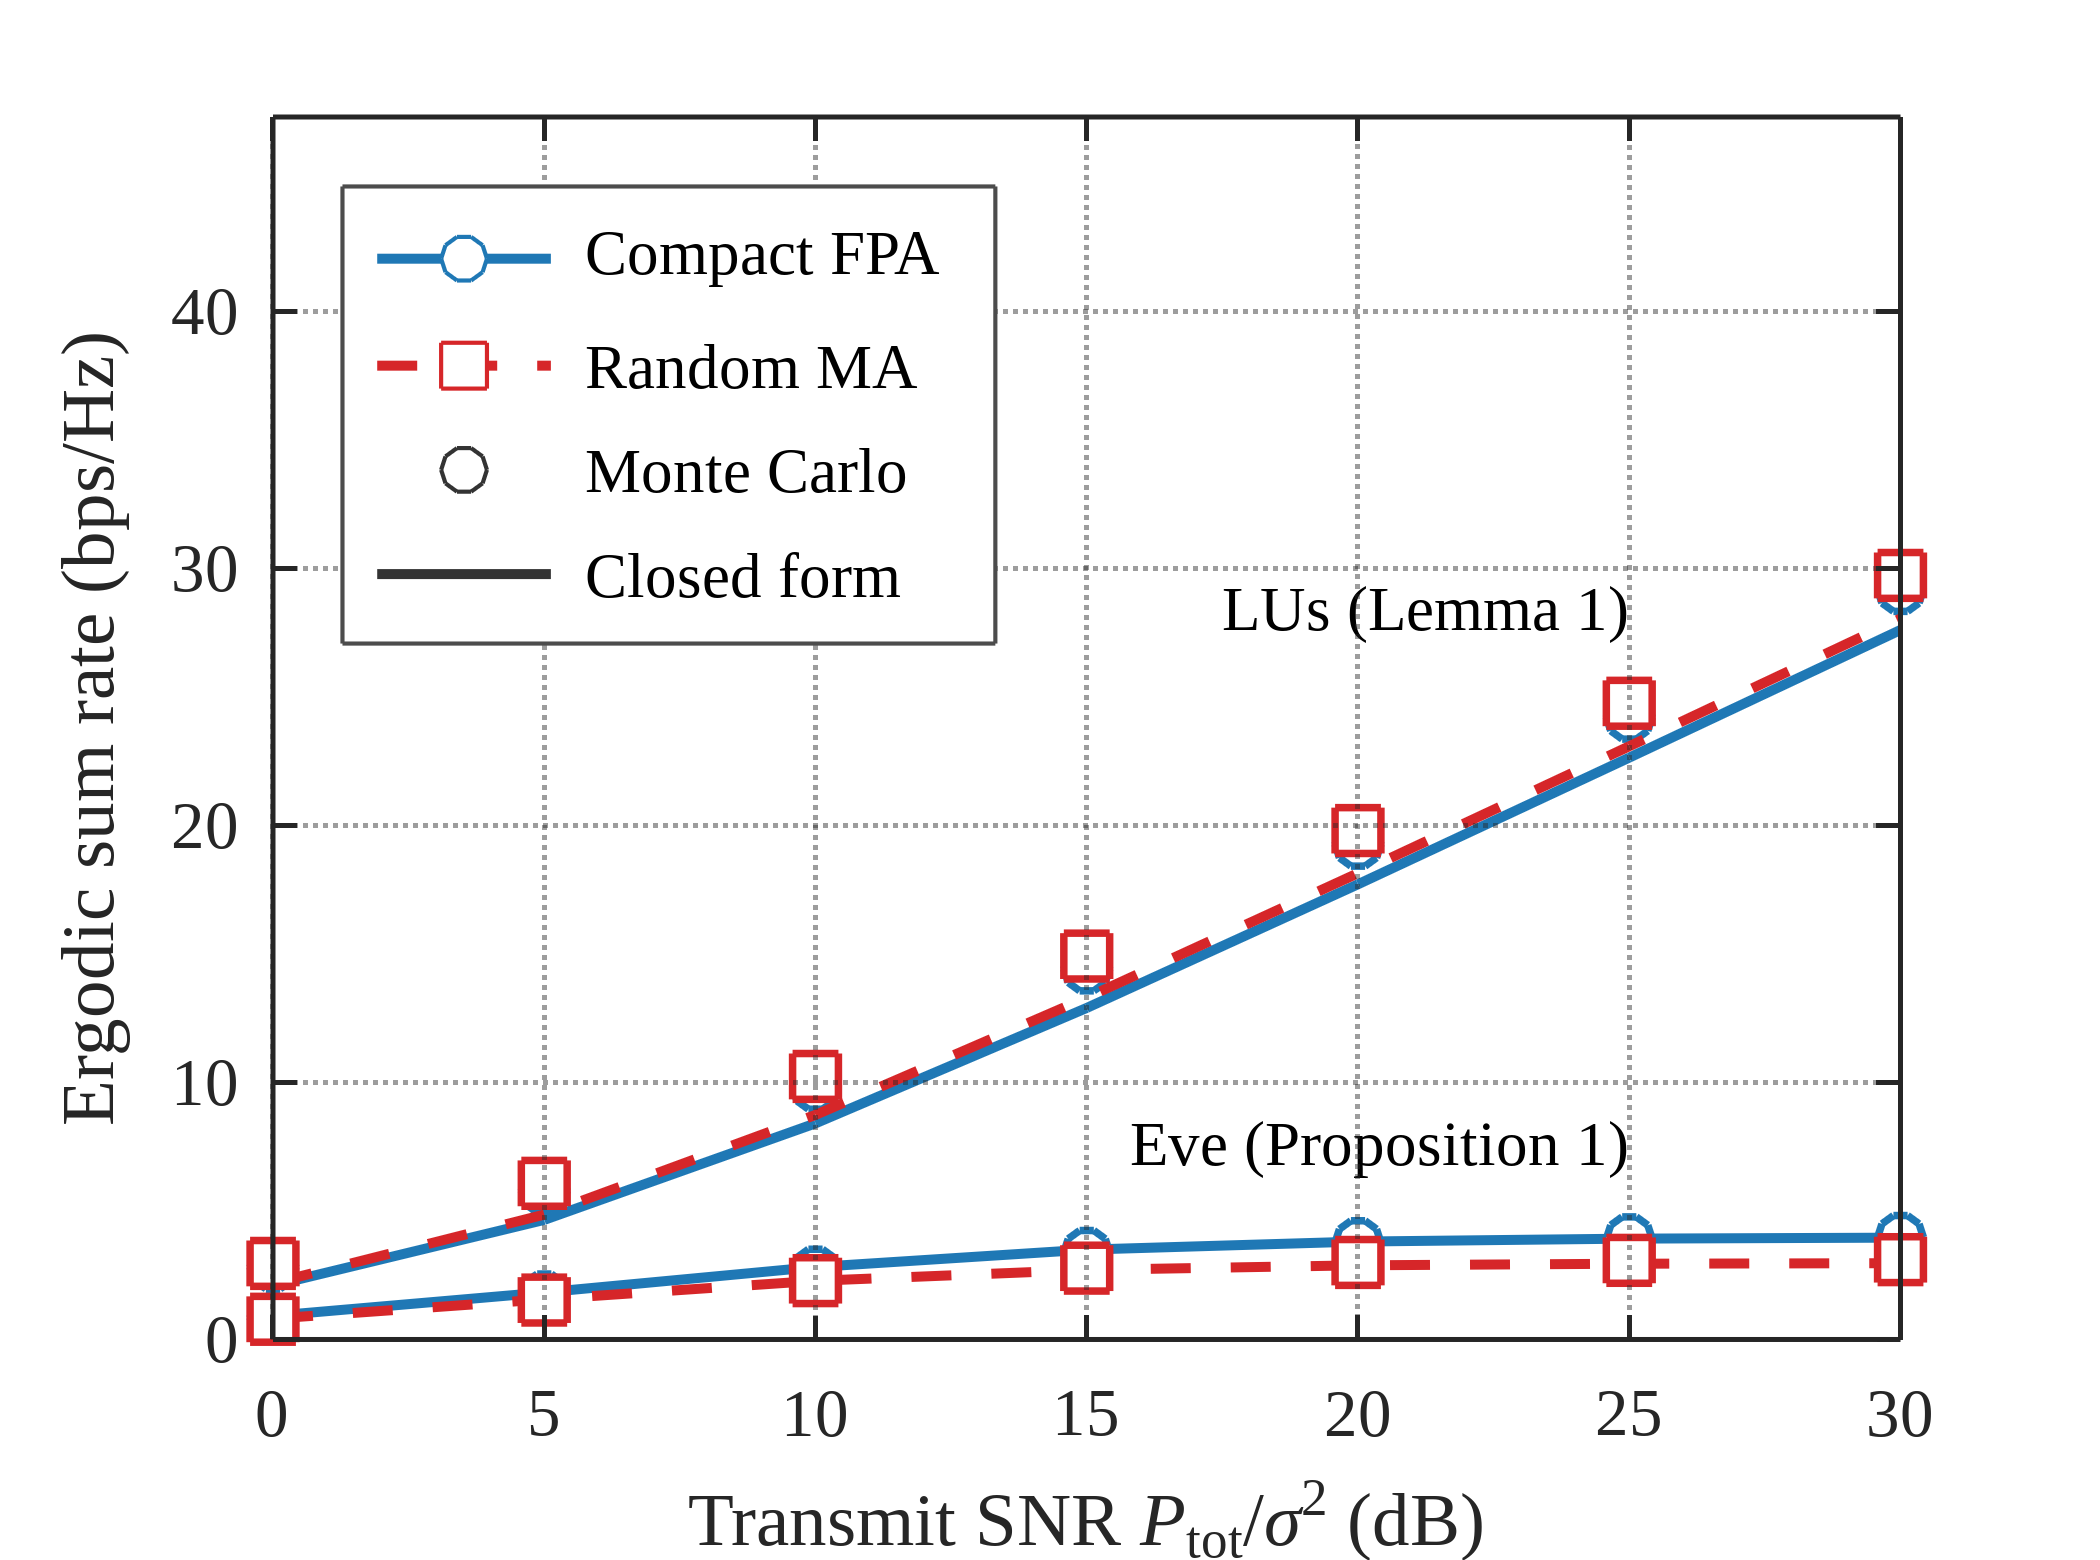
\includegraphics[width=0.48\textwidth]{fig3a_accuracy_snr}\label{fig:acc_P}}\hfil
\subfloat[]{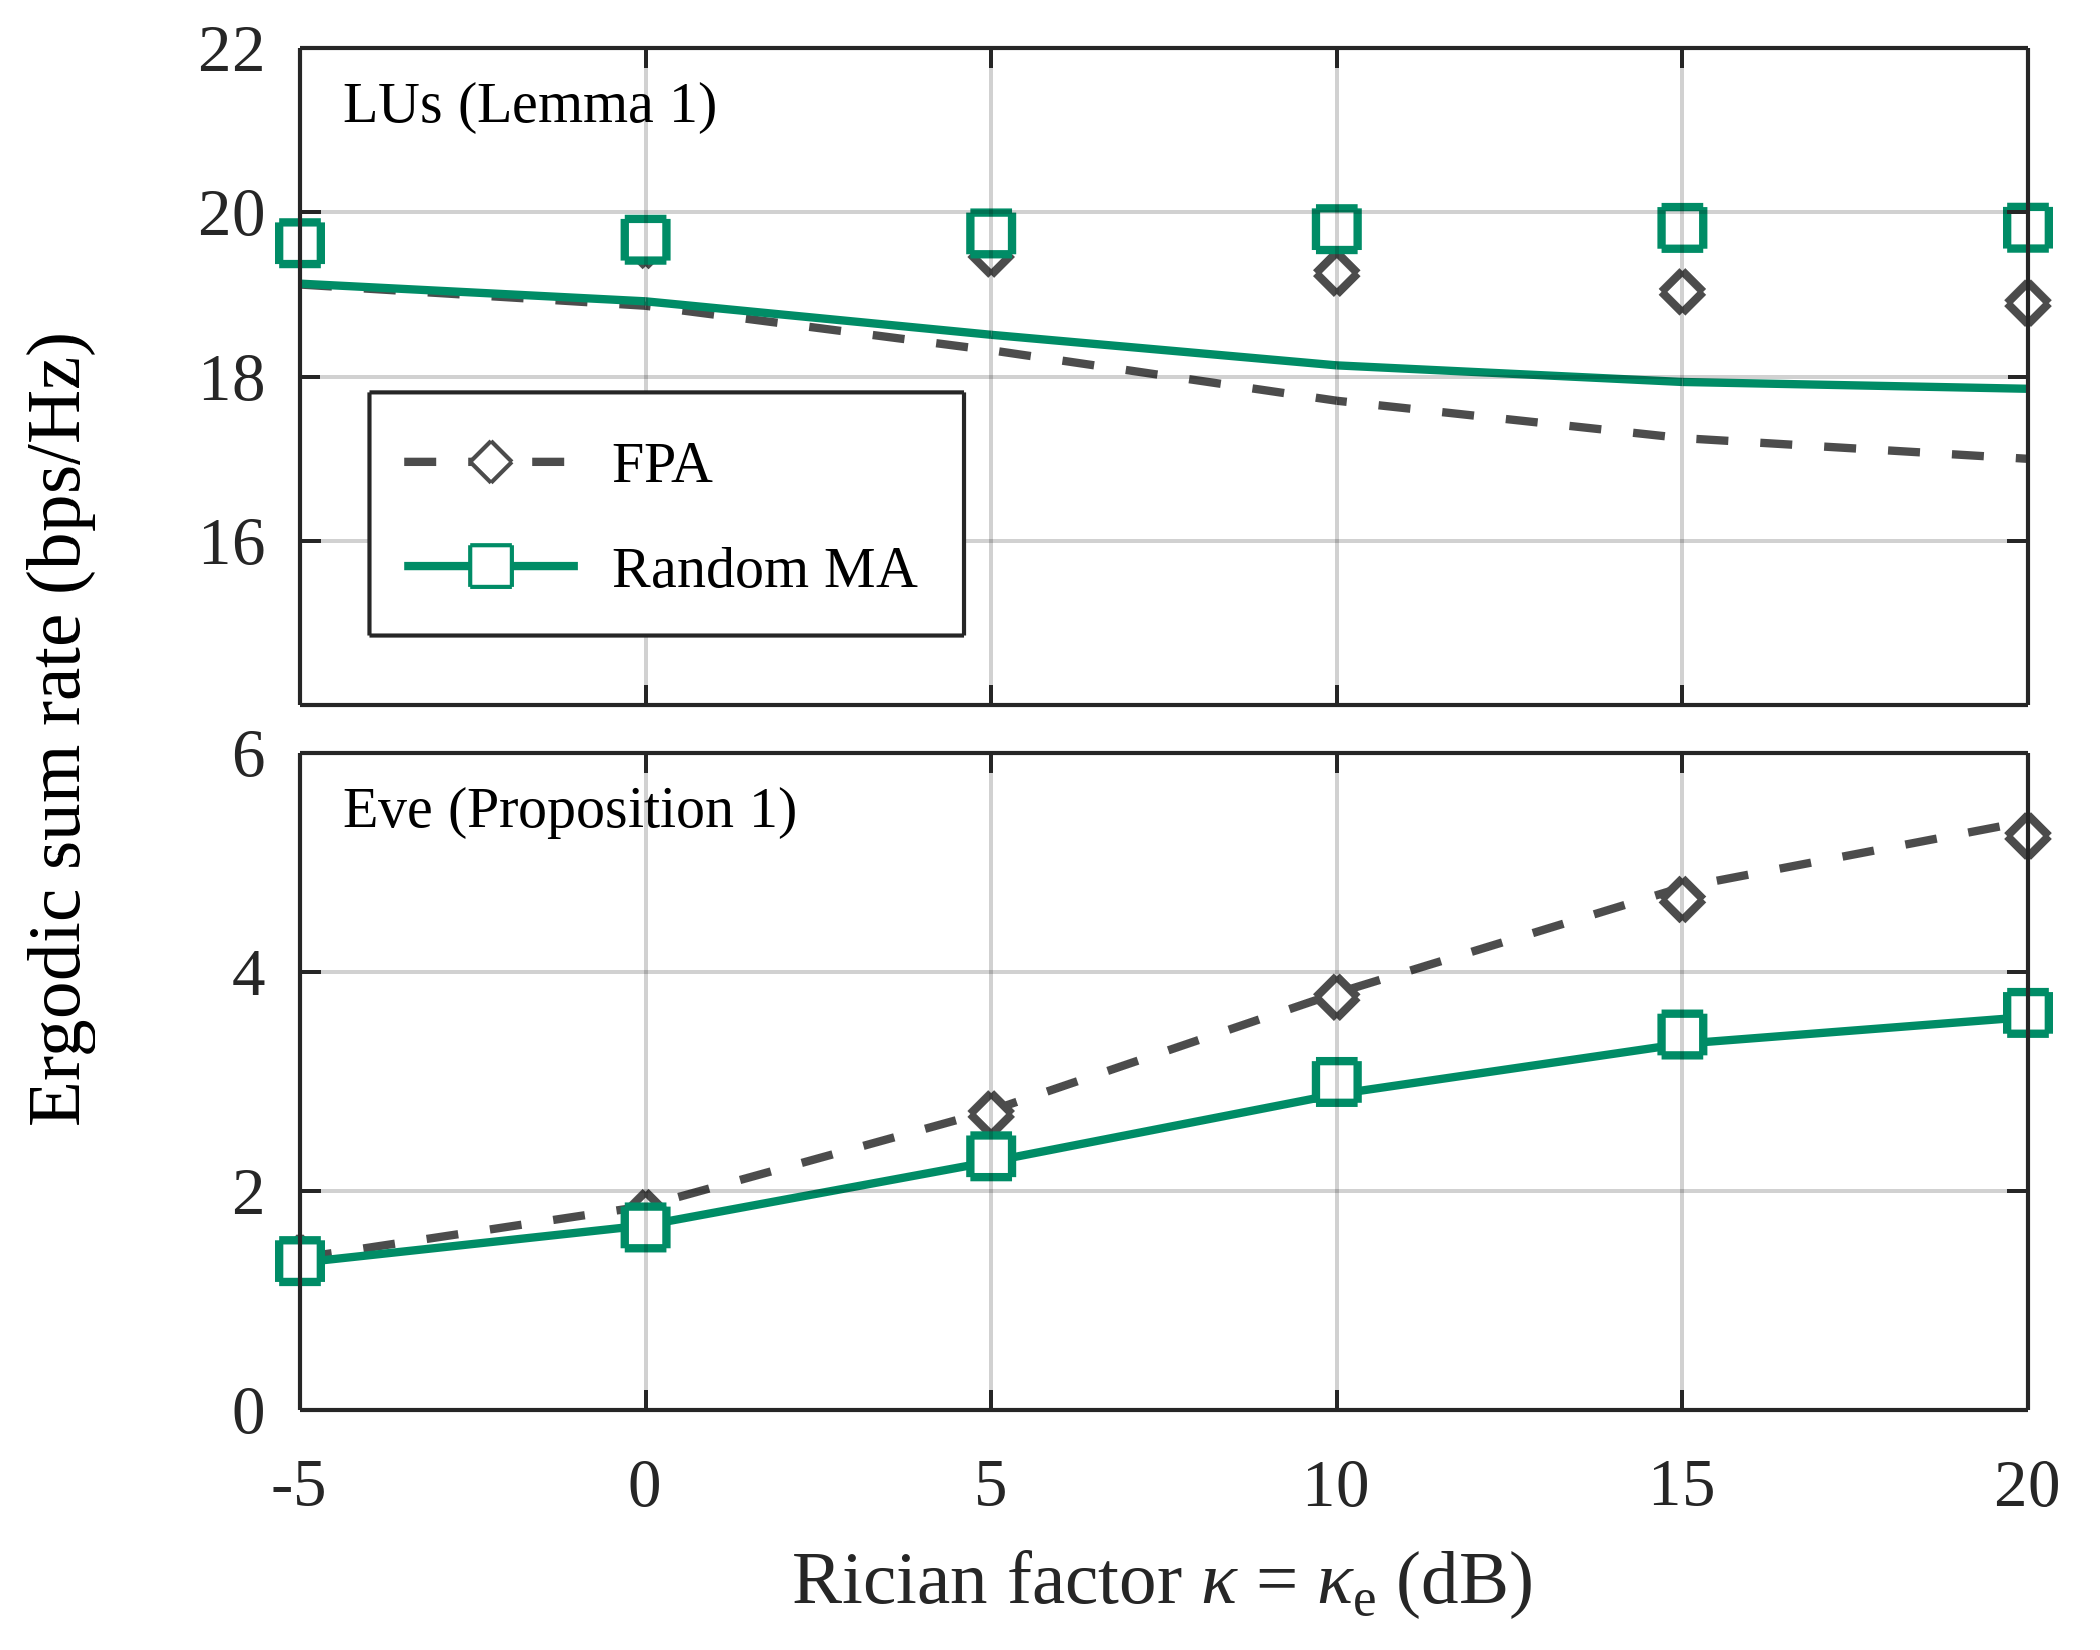
\includegraphics[width=0.48\textwidth]{fig3b_accuracy_kappa}\label{fig:acc_K}}
\caption{Ergodic sum rates of the LUs (upper panels) and Eve (lower panels) with $p_m=\Ptot/(2M)$ and $q=\Ptot/(2(N-M))$: (a) versus the transmit SNR with $\kappa=\kappa_e=10$~dB; (b) versus the Rician factor with $\Ptot/\sigma^2=20$~dB. Lines: closed-form approximations; markers: Monte Carlo simulations.}
\label{fig:acc}
\end{figure*}

Fig.~\ref{fig:acc} evaluates the accuracy of Lemma~\ref{lem:lu} and Proposition~\ref{prop:eve} for the FPA and for random feasible MA positions, where the power is split equally between the confidential signals and the AN, i.e., $\alpha=0.5$ in Remark~\ref{rem:highsnr}. The closed-form ergodic wiretap rate in Proposition~\ref{prop:eve} agrees well with the Monte Carlo results over the entire ranges of the SNR and the Rician factor, with a maximum error of 0.16~bps/Hz in the ergodic wiretap sum rate. In particular, the error is negligible in the NLoS-dominant regime, e.g., for $\kappa=-5$~dB, where Lemma~\ref{lem:det} is exact, and remains small in the LoS-dominant regime. Moreover, the random MA positions yield a lower wiretap rate than the FPA, since their larger aperture reduces the LoS correlation between Eve and LU~1. As discussed in Remark~\ref{rem:lu}, Lemma~\ref{lem:lu} underestimates the ergodic rates of the LUs, and the gap increases with the Rician factor. Nevertheless, the gap is almost the same for the two configurations, e.g., 1.55 and 1.66~bps/Hz at $\kappa=10$~dB and $\Ptot/\sigma^2=20$~dB. More importantly, at the designs obtained in Fig.~\ref{fig:snr}(a) for $\Ptot/\sigma^2=20$~dB, the Monte Carlo ESSR exceeds the approximate ESSR in~\eqref{eq:esrapprox} by 1.52--1.73~bps/Hz for all the schemes, so that the relative gains of the proposed design predicted by~\eqref{eq:esrapprox} deviate from the Monte Carlo ones by at most 2.2 percentage points. Hence, the conservative approximation preserves the ranking of the antenna designs.

\subsection{Convergence of Algorithm~\ref{alg:ao}}

\begin{figure}[t]
\centering
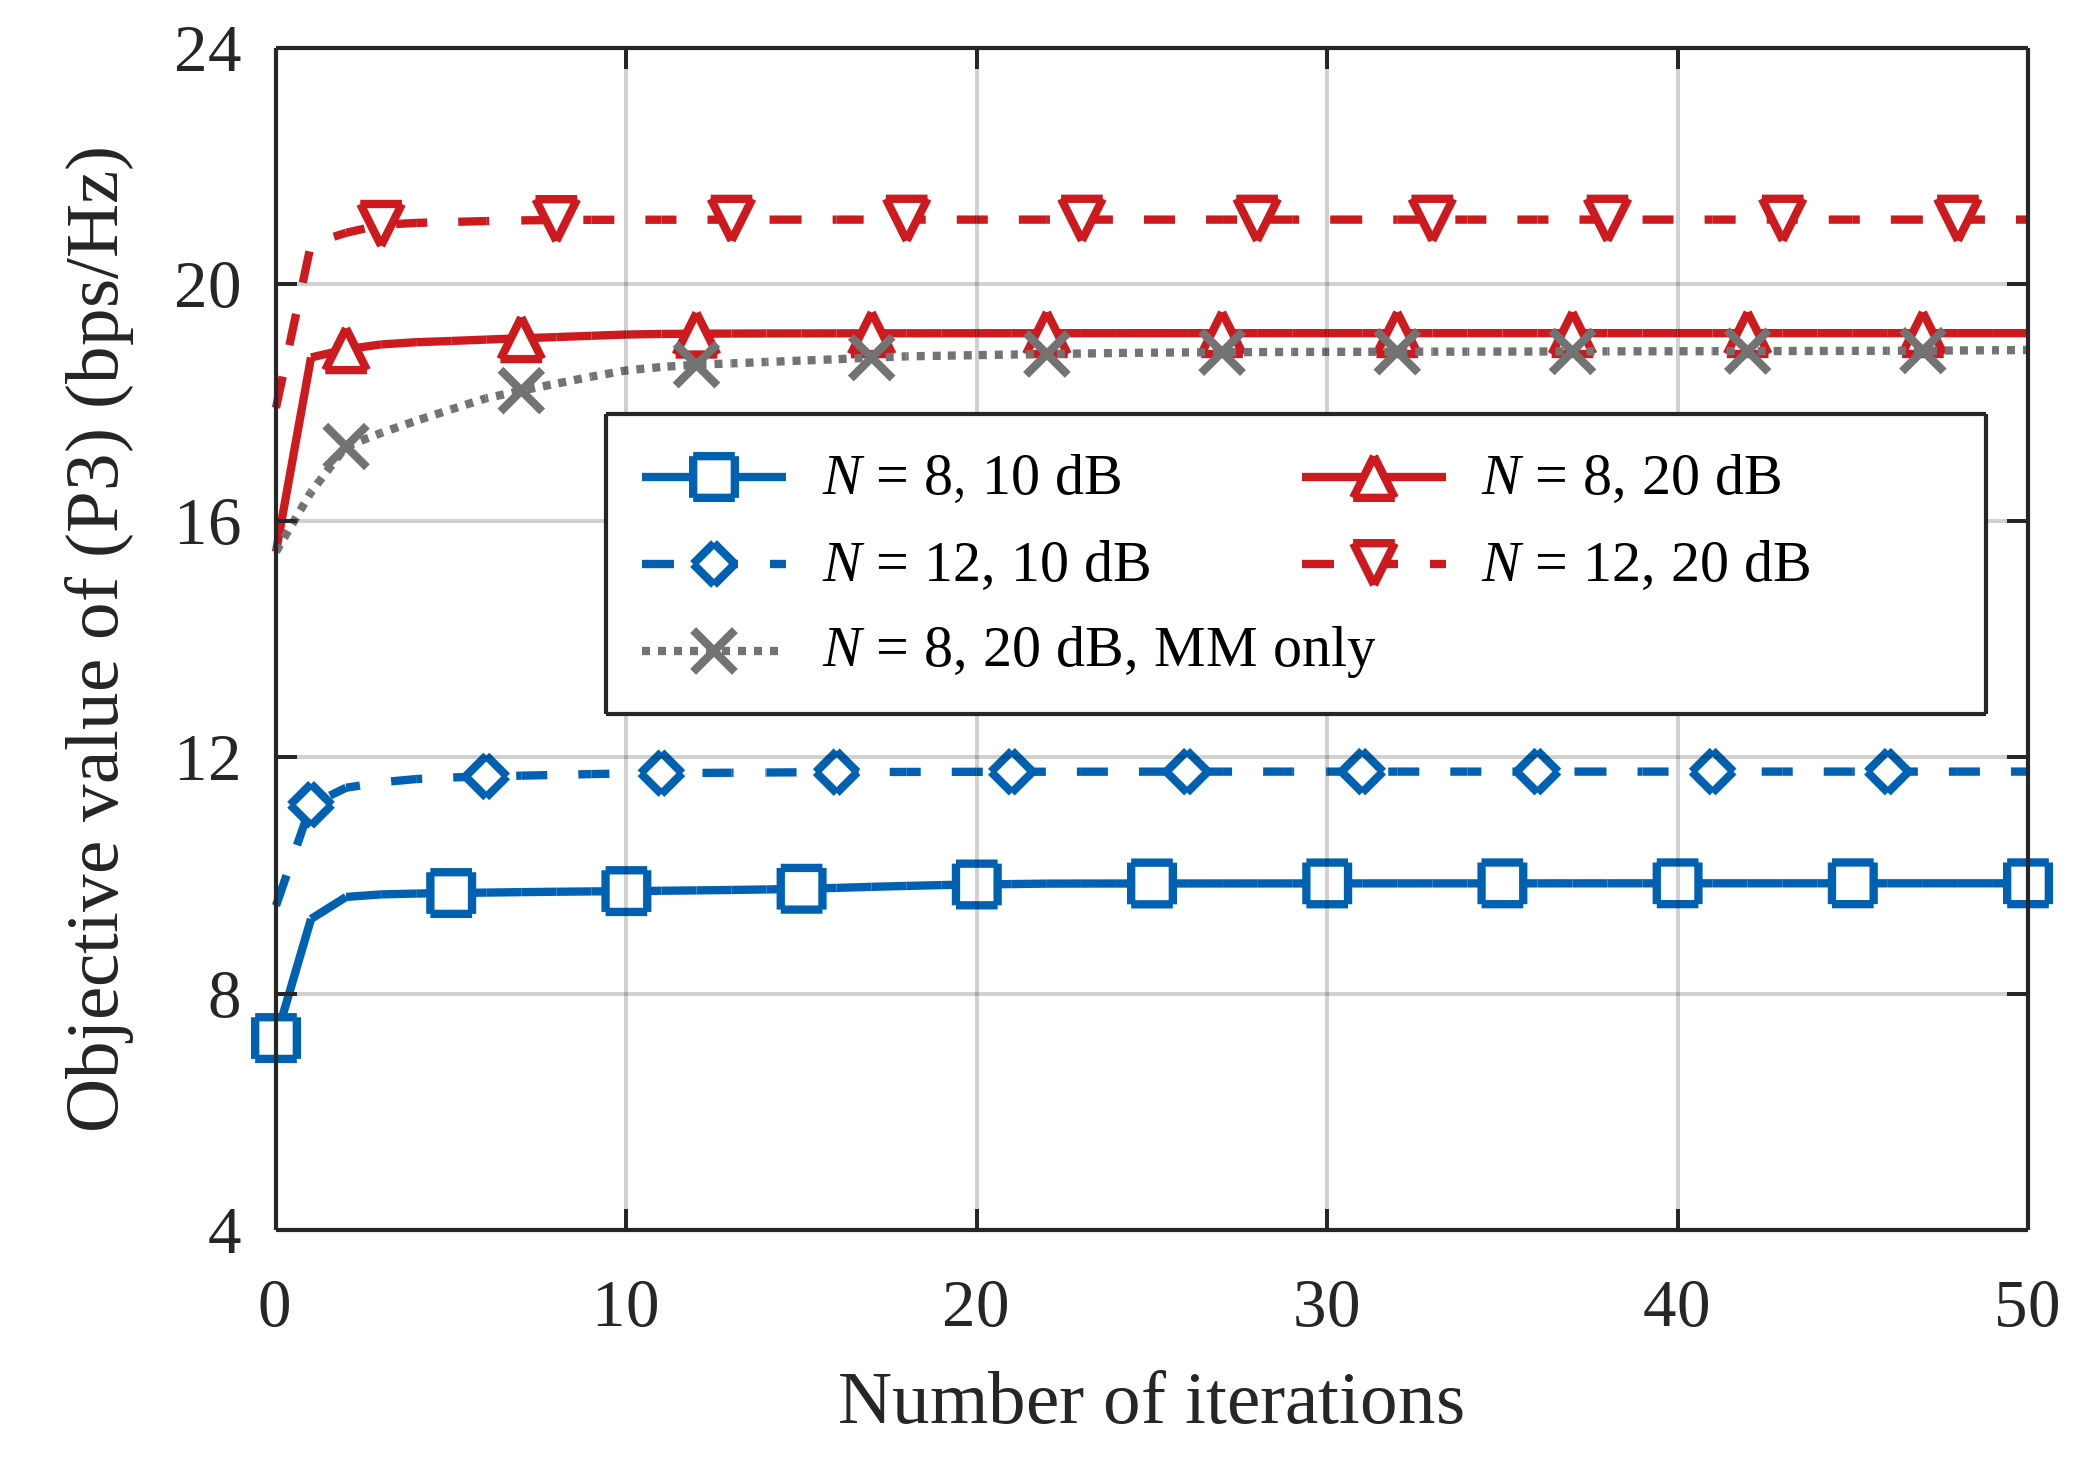
\includegraphics[width=\columnwidth]{fig4_convergence}
\caption{Convergence of Algorithm~\ref{alg:ao} for one realization of the AoDs and three initializations ($\Ptot/\sigma^2=20$~dB).}
\label{fig:conv}
\end{figure}

Fig.~\ref{fig:conv} shows the objective value of (P3) versus the number of iterations of Algorithm~\ref{alg:ao} for one realization of the AoDs and three initializations, where the stopping criterion is disabled to show the complete trajectories. The objective value increases monotonically, which verifies the convergence analysis in Section~\ref{sec:opt}-D. About $28\%$--$44\%$ of the total improvement is achieved in the first iteration, and $95\%$ within $29$--$41$ iterations. With $\epsilon=10^{-4}$, Algorithm~\ref{alg:ao} terminates after $38$--$50$ iterations. The final objective values of the three initializations differ by at most 4.5\%, and the UPA initialization yields the best one. Similar behavior is observed at $\Ptot/\sigma^2=10$ and $30$~dB, where $95\%$ of the improvement is attained within $25$--$57$ iterations and the UPA initialization again performs best, which indicates that a few initializations suffice in practice.

\subsection{ESSR and AN Power Versus Transmit SNR}

\begin{figure*}[t]
\centering
\subfloat[]{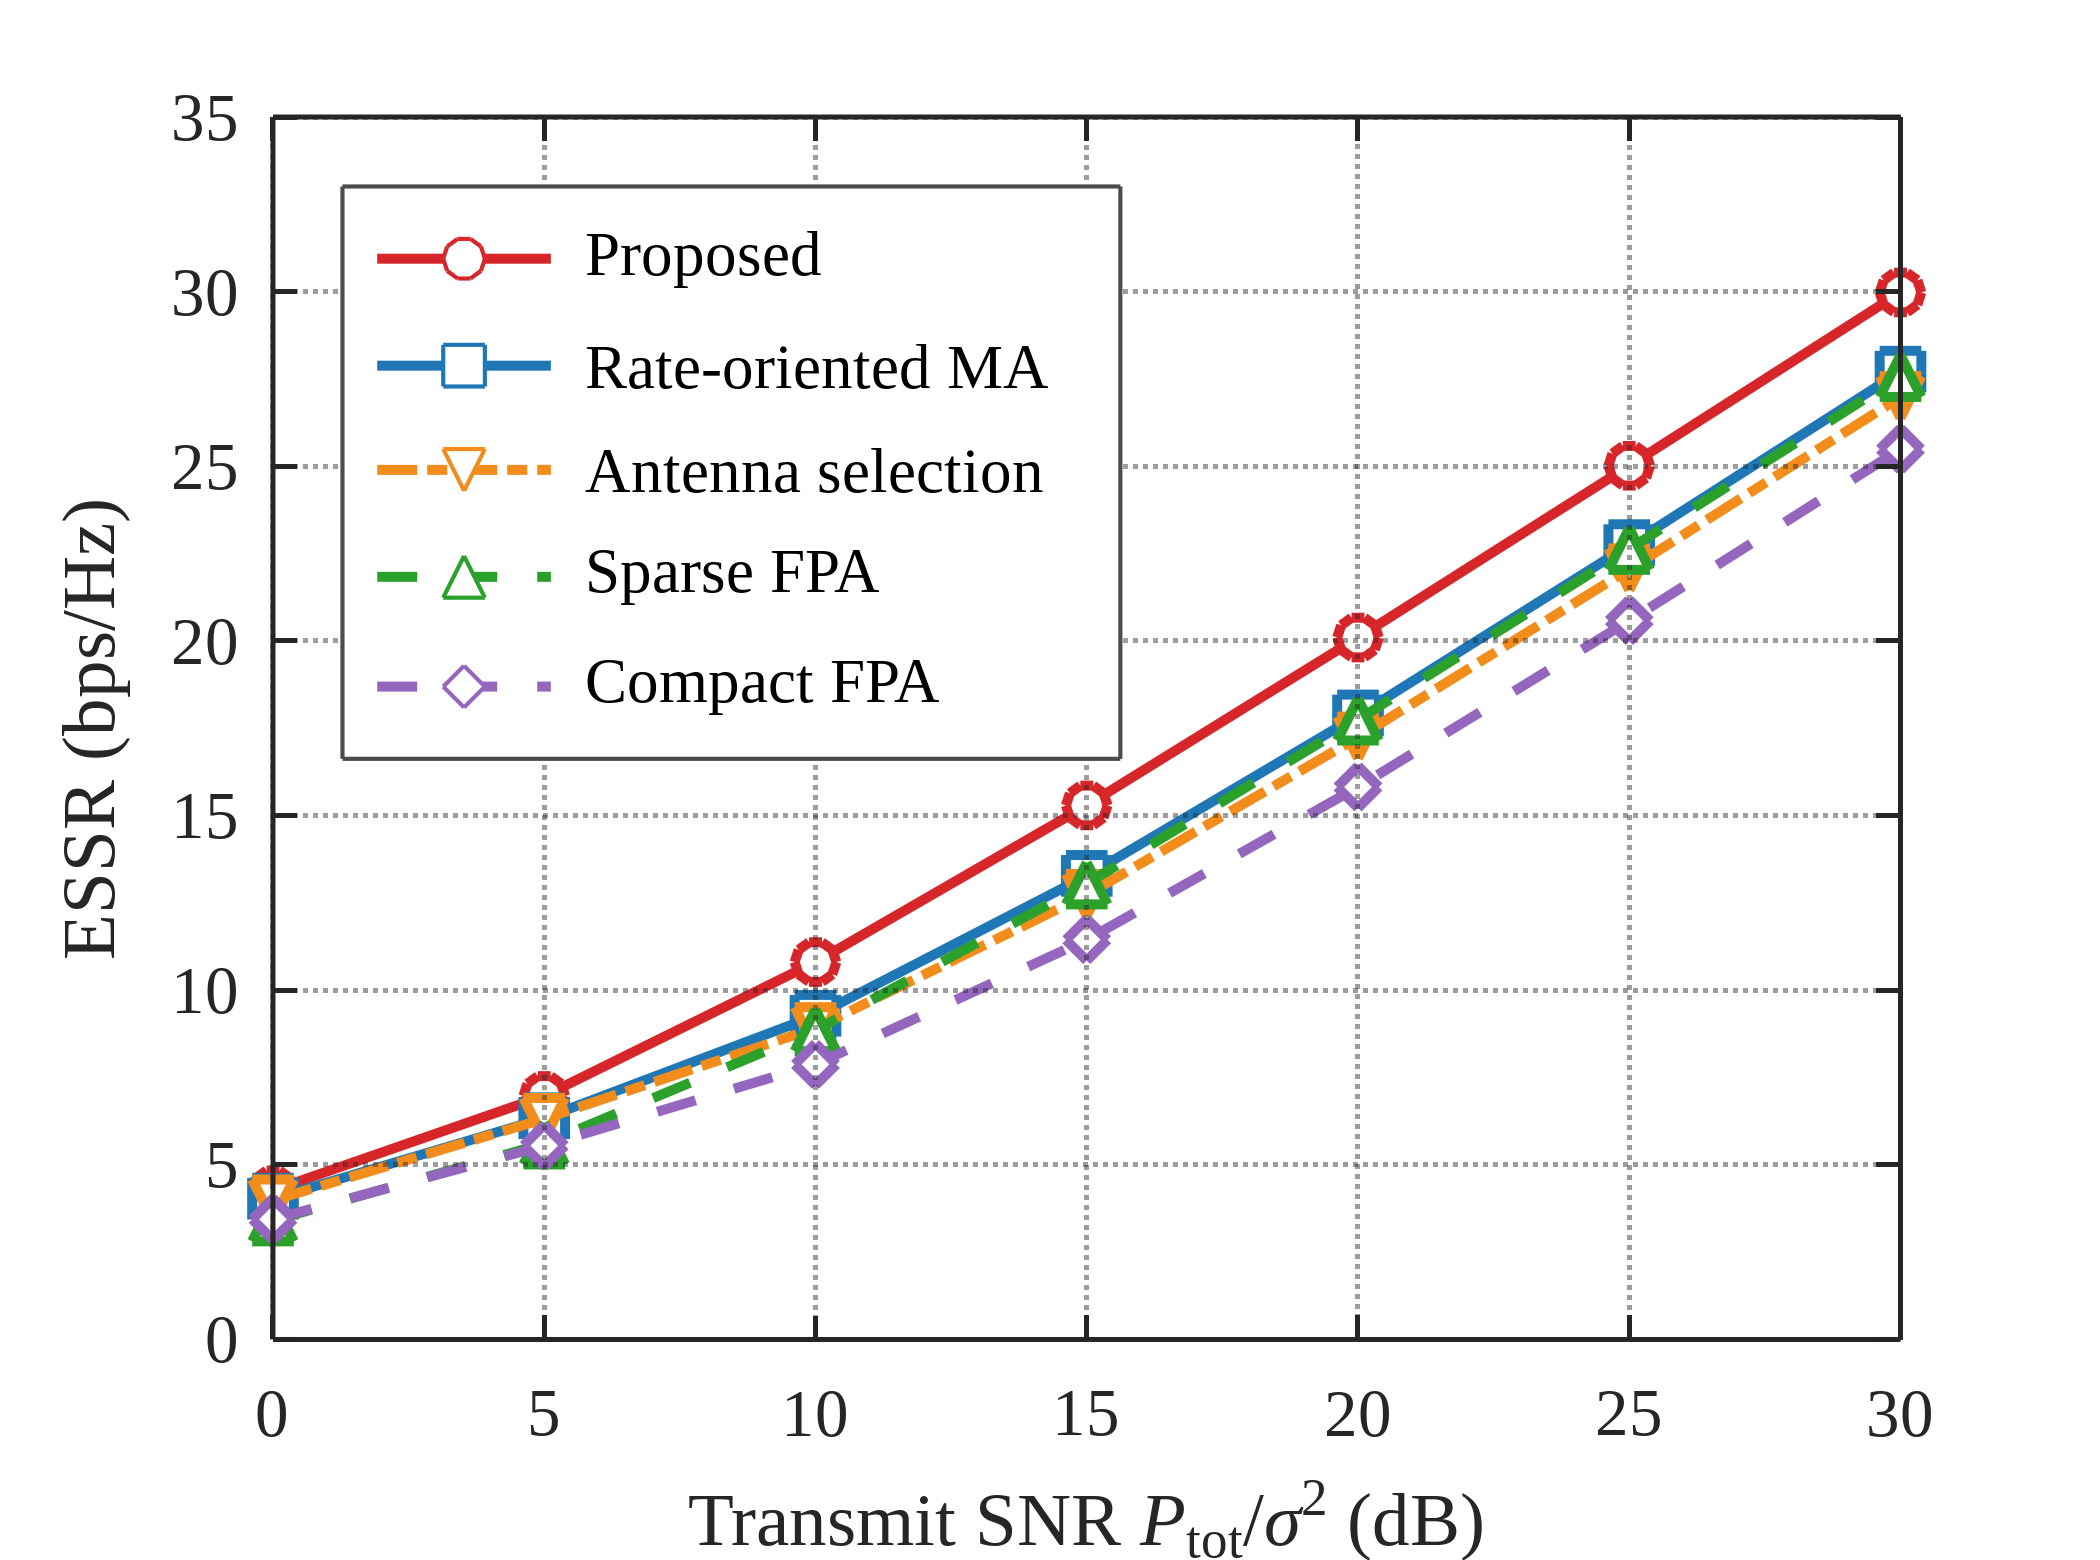
\includegraphics[width=0.48\textwidth]{fig5a_essr_snr}\label{fig:snr_essr}}\hfil
\subfloat[]{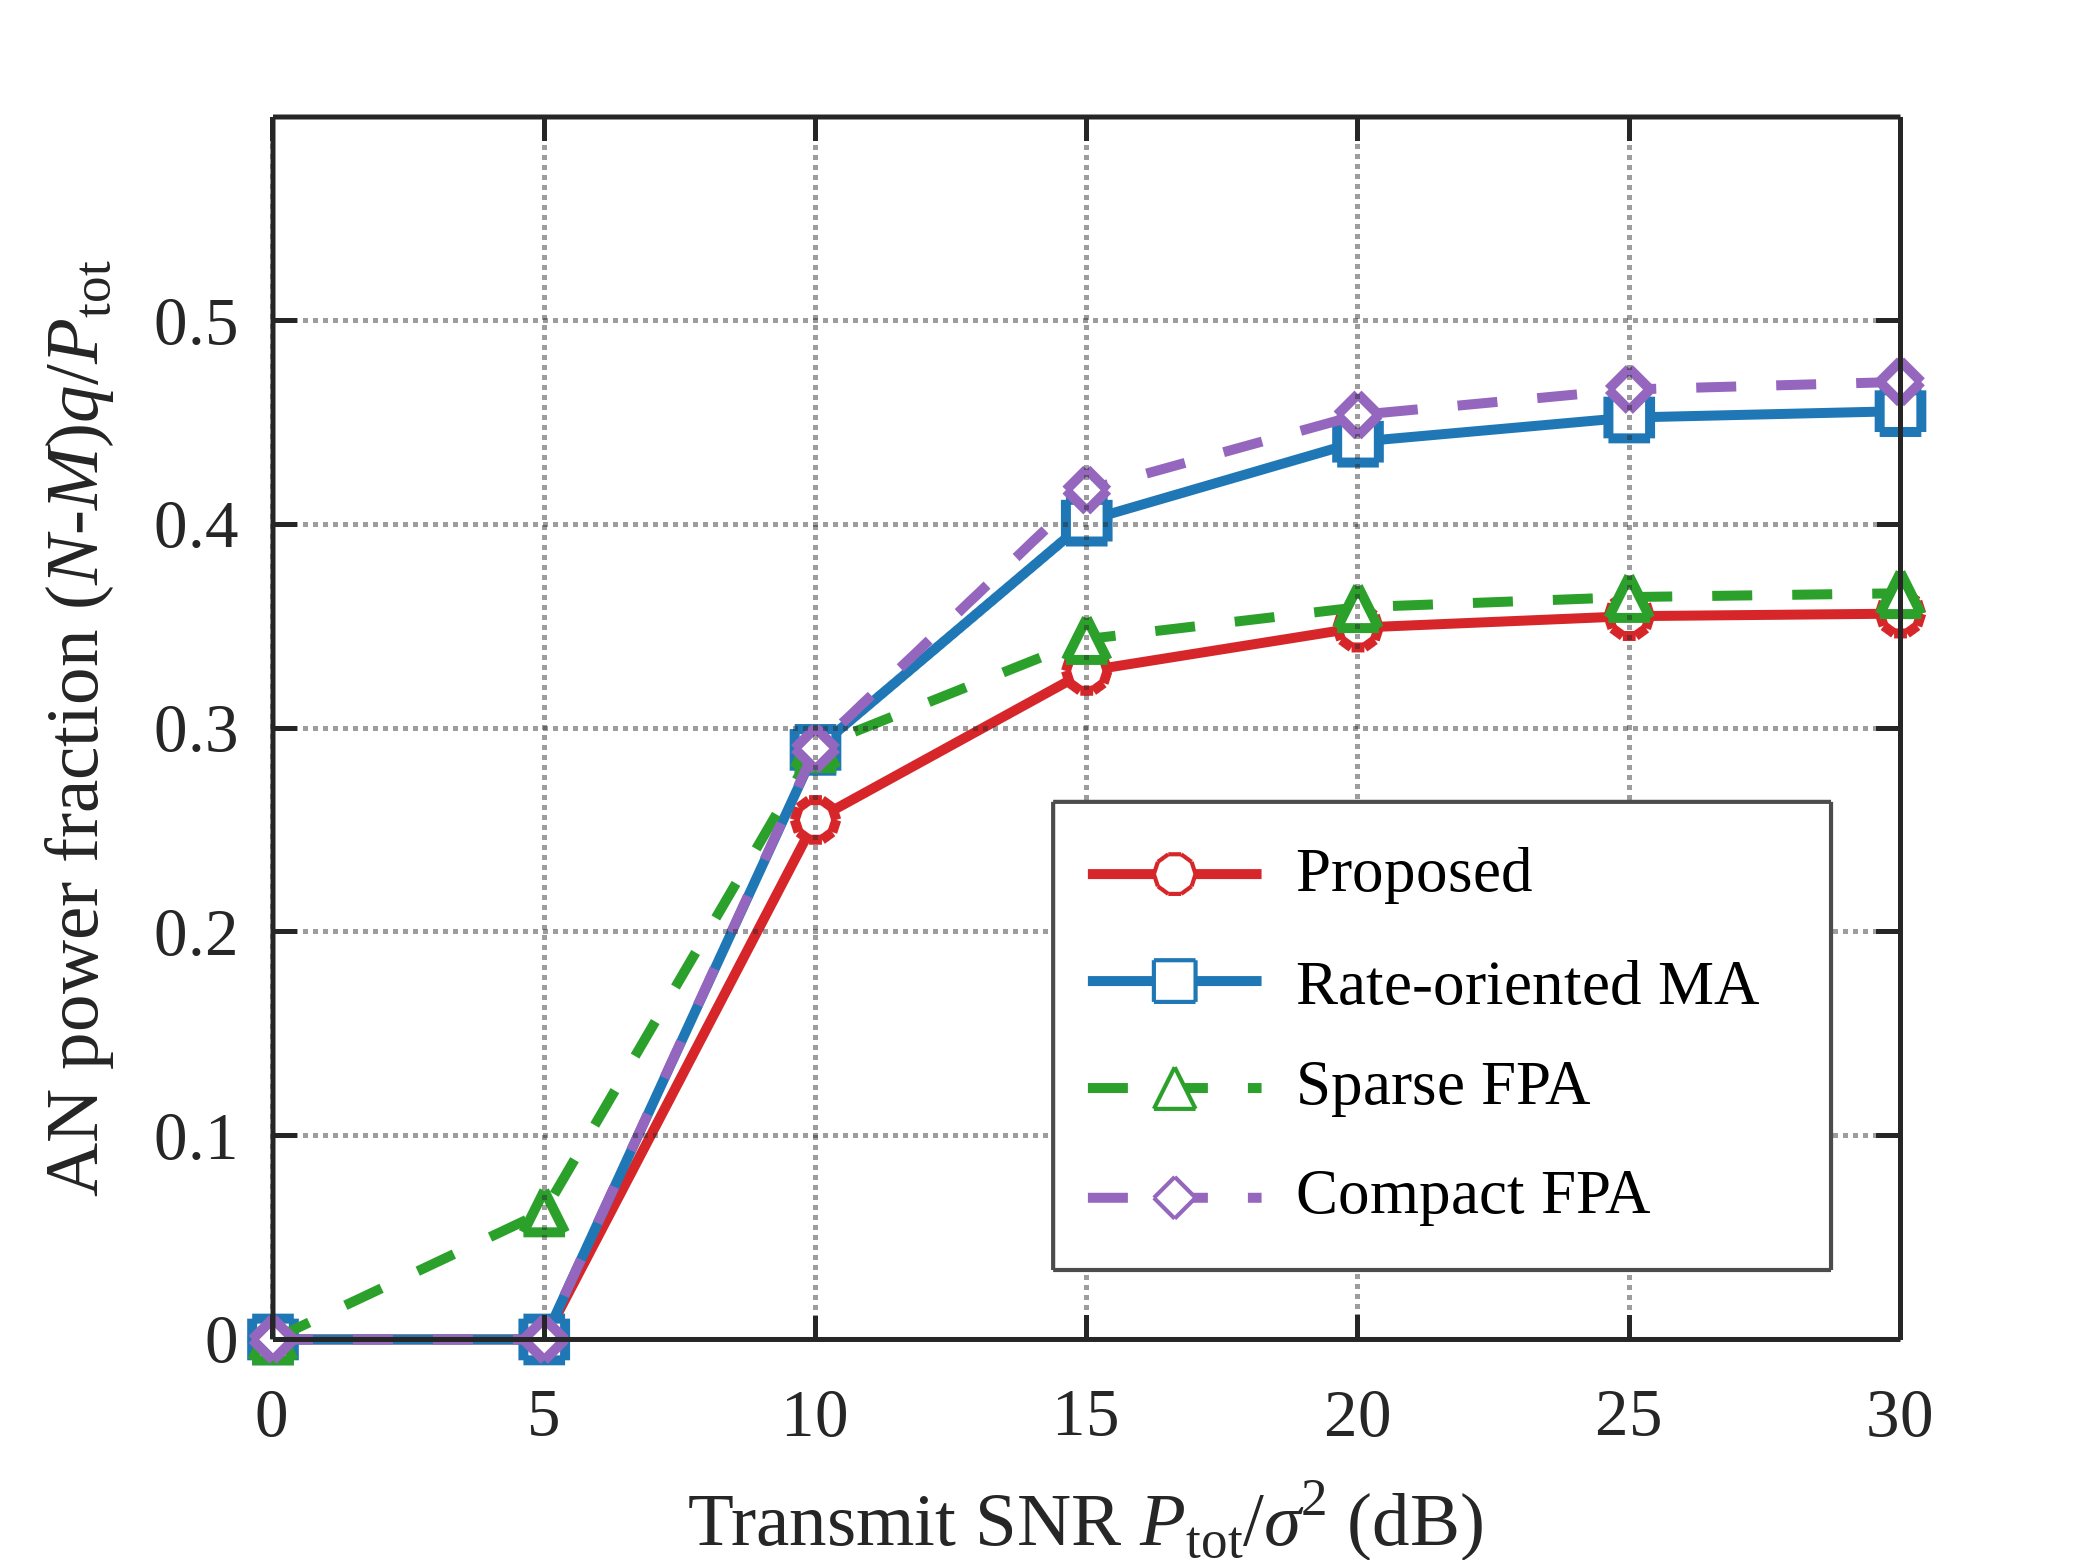
\includegraphics[width=0.48\textwidth]{fig5b_an_fraction}\label{fig:snr_an}}
\caption{(a) ESSR and (b) optimized AN power fraction $(N-M)q/\Ptot$ versus the transmit SNR.}
\label{fig:snr}
\end{figure*}

\begin{table}[t]
\caption{ESSR (bps/Hz) Under Different Eavesdropper Models}
\label{tab:eve}
\centering
\footnotesize
\setlength{\tabcolsep}{4.2pt}
\renewcommand{\arraystretch}{1.12}
\begin{tabular}{lcccccc}
\hline
 & \multicolumn{3}{c}{Worst-case Eve~\eqref{eq:sinre_gen}} & \multicolumn{3}{c}{TIN Eve~\eqref{eq:sinre_tin}}\\
$\Ptot/\sigma^2$ (dB) & $10$ & $20$ & $30$ & $10$ & $20$ & $30$\\
\hline
Proposed & \textbf{10.81} & \textbf{20.10} & \textbf{29.98} & \textbf{11.35} & \textbf{20.73} & \textbf{30.62}\\
Rate-oriented MA & 9.27 & 17.87 & 27.71 & 10.40 & 19.39 & 29.25\\
AS & 8.92 & 17.24 & 26.98 & 9.77 & 18.58 & 28.39\\
FPA & 7.88 & 15.82 & 25.49 & 8.70 & 17.24 & 27.00\\
Proposed w/o AN & 9.33 & 12.13 & 12.94 & 10.39 & 17.75 & 26.06\\
\hline
\end{tabular}
\end{table}

Fig.~\ref{fig:snr}(a) shows that the proposed design achieves the highest ESSR over the entire SNR range. At $\Ptot/\sigma^2=20$~dB, it improves the ESSR by 12.5\%, 16.6\%, and 27.1\% compared with the rate-oriented MA, AS, and the FPA, respectively, and outperforms each of them in every one of the $100$ AoD realizations. Although the rate-oriented MA exploits the same region, it achieves less than half of the gain of the proposed design over the FPA, i.e., the secrecy gain stems mainly from the Eve-aware positioning enabled by Proposition~\ref{prop:eve} rather than from the decorrelation among the LUs. AS improves the ESSR over the FPA by only 9.0\%, although it uses the same metric as the proposed design with twice as many antennas, since its candidates are restricted to a $\lambda/2$-spaced grid with an aperture of $1.5\lambda\times1.5\lambda$. As the SNR increases, the gains of the proposed design over the FPA and the rate-oriented MA saturate at about 4.5 and 2.3~bps/Hz, respectively, which agrees with Remark~\ref{rem:highsnr}: the antenna positions do not change the high-SNR slope of the ESSR but improve its constant term.

Fig.~\ref{fig:snr}(b) shows the optimized AN power fraction, which increases with the SNR and saturates at high SNR, in agreement with~\eqref{eq:alphastar}. The proposed design requires considerably less AN power than all the benchmarks, e.g., 0.31 versus 0.44, 0.43, and 0.47 for the rate-oriented MA, AS, and the FPA, respectively, at $\Ptot/\sigma^2=20$~dB, whereas the rate-oriented MA saves little AN power compared with the FPA. This verifies the AN-saving effect in Remark~\ref{rem:highsnr}: by decorrelating the LoS component of Eve from those of the LUs, the proposed positions reduce the information leakage and increase the AN received by Eve, so that more power can be allocated to the confidential signals.

Table~\ref{tab:eve} examines the impact of the worst-case model in~\eqref{eq:sinre_gen} by also evaluating the obtained designs, all of which are optimized under~\eqref{eq:sinre_gen}, against an Eve that treats the signals of the other LUs as interference (TIN), whose SINR is
\begin{equation}\label{eq:sinre_tin}
\gamma_{e,m}^{\mathrm{TIN}}=\frac{p_m|\bg^H\wb_m|^2}{\sum_{i\in\mathcal M\setminus\{m\}}p_i|\bg^H\wb_i|^2+q\,\bg^H\PHp\bg+\sigma_e^2}.
\end{equation}
First, the proposed design achieves the highest ESSR under both models, and its ESSR under the worst-case model is only 3.0\% lower than that against the TIN Eve at $\Ptot/\sigma^2=20$~dB, i.e., the secrecy guarantee of the worst-case model comes at a marginal cost. Second, without AN, the ESSR strongly depends on the eavesdropper model: against the TIN Eve, the inter-user interference acts as AN, and the ESSR increases with the SNR, whereas under the worst-case model it saturates at about 13~bps/Hz~\cite{Goel2008}. Hence, the AN is indispensable for a secrecy performance that does not rely on the decoding capability of Eve. Third, against the TIN Eve, the proposed design still outperforms the rate-oriented MA and the FPA by 6.9\% and 20.2\% at $20$~dB, respectively. These gains are smaller than under the worst-case model, since the inter-user interference partially masks the higher information leakage of the benchmarks, but they confirm that the gain is not an artifact of the worst-case assumption.

Finally, we examine the robustness to imperfect statistical CSI of Eve, where all the schemes are designed with an AoD of Eve that deviates from the true one by $\varepsilon$ in a random direction and are evaluated with the true AoD. For $\varepsilon=0.01$, $0.02$, and $0.05$~rad, the ESSR of the proposed design at $20$~dB decreases by only 0.2\%, 0.3\%, and 2.2\%, respectively, and its gain over the rate-oriented MA remains above 10\%. Even for $\varepsilon=\Delta=0.1$~rad, i.e., an error as large as the angular offset between Eve and LU~1, the proposed design still outperforms all the benchmarks, e.g., by 3.8\% compared with the rate-oriented MA. Hence, the proposed design is robust to moderate errors in the AoD of Eve.

\subsection{Region Size, Angular Offset, and Single-LU Case}

\begin{figure}[t]
\centering
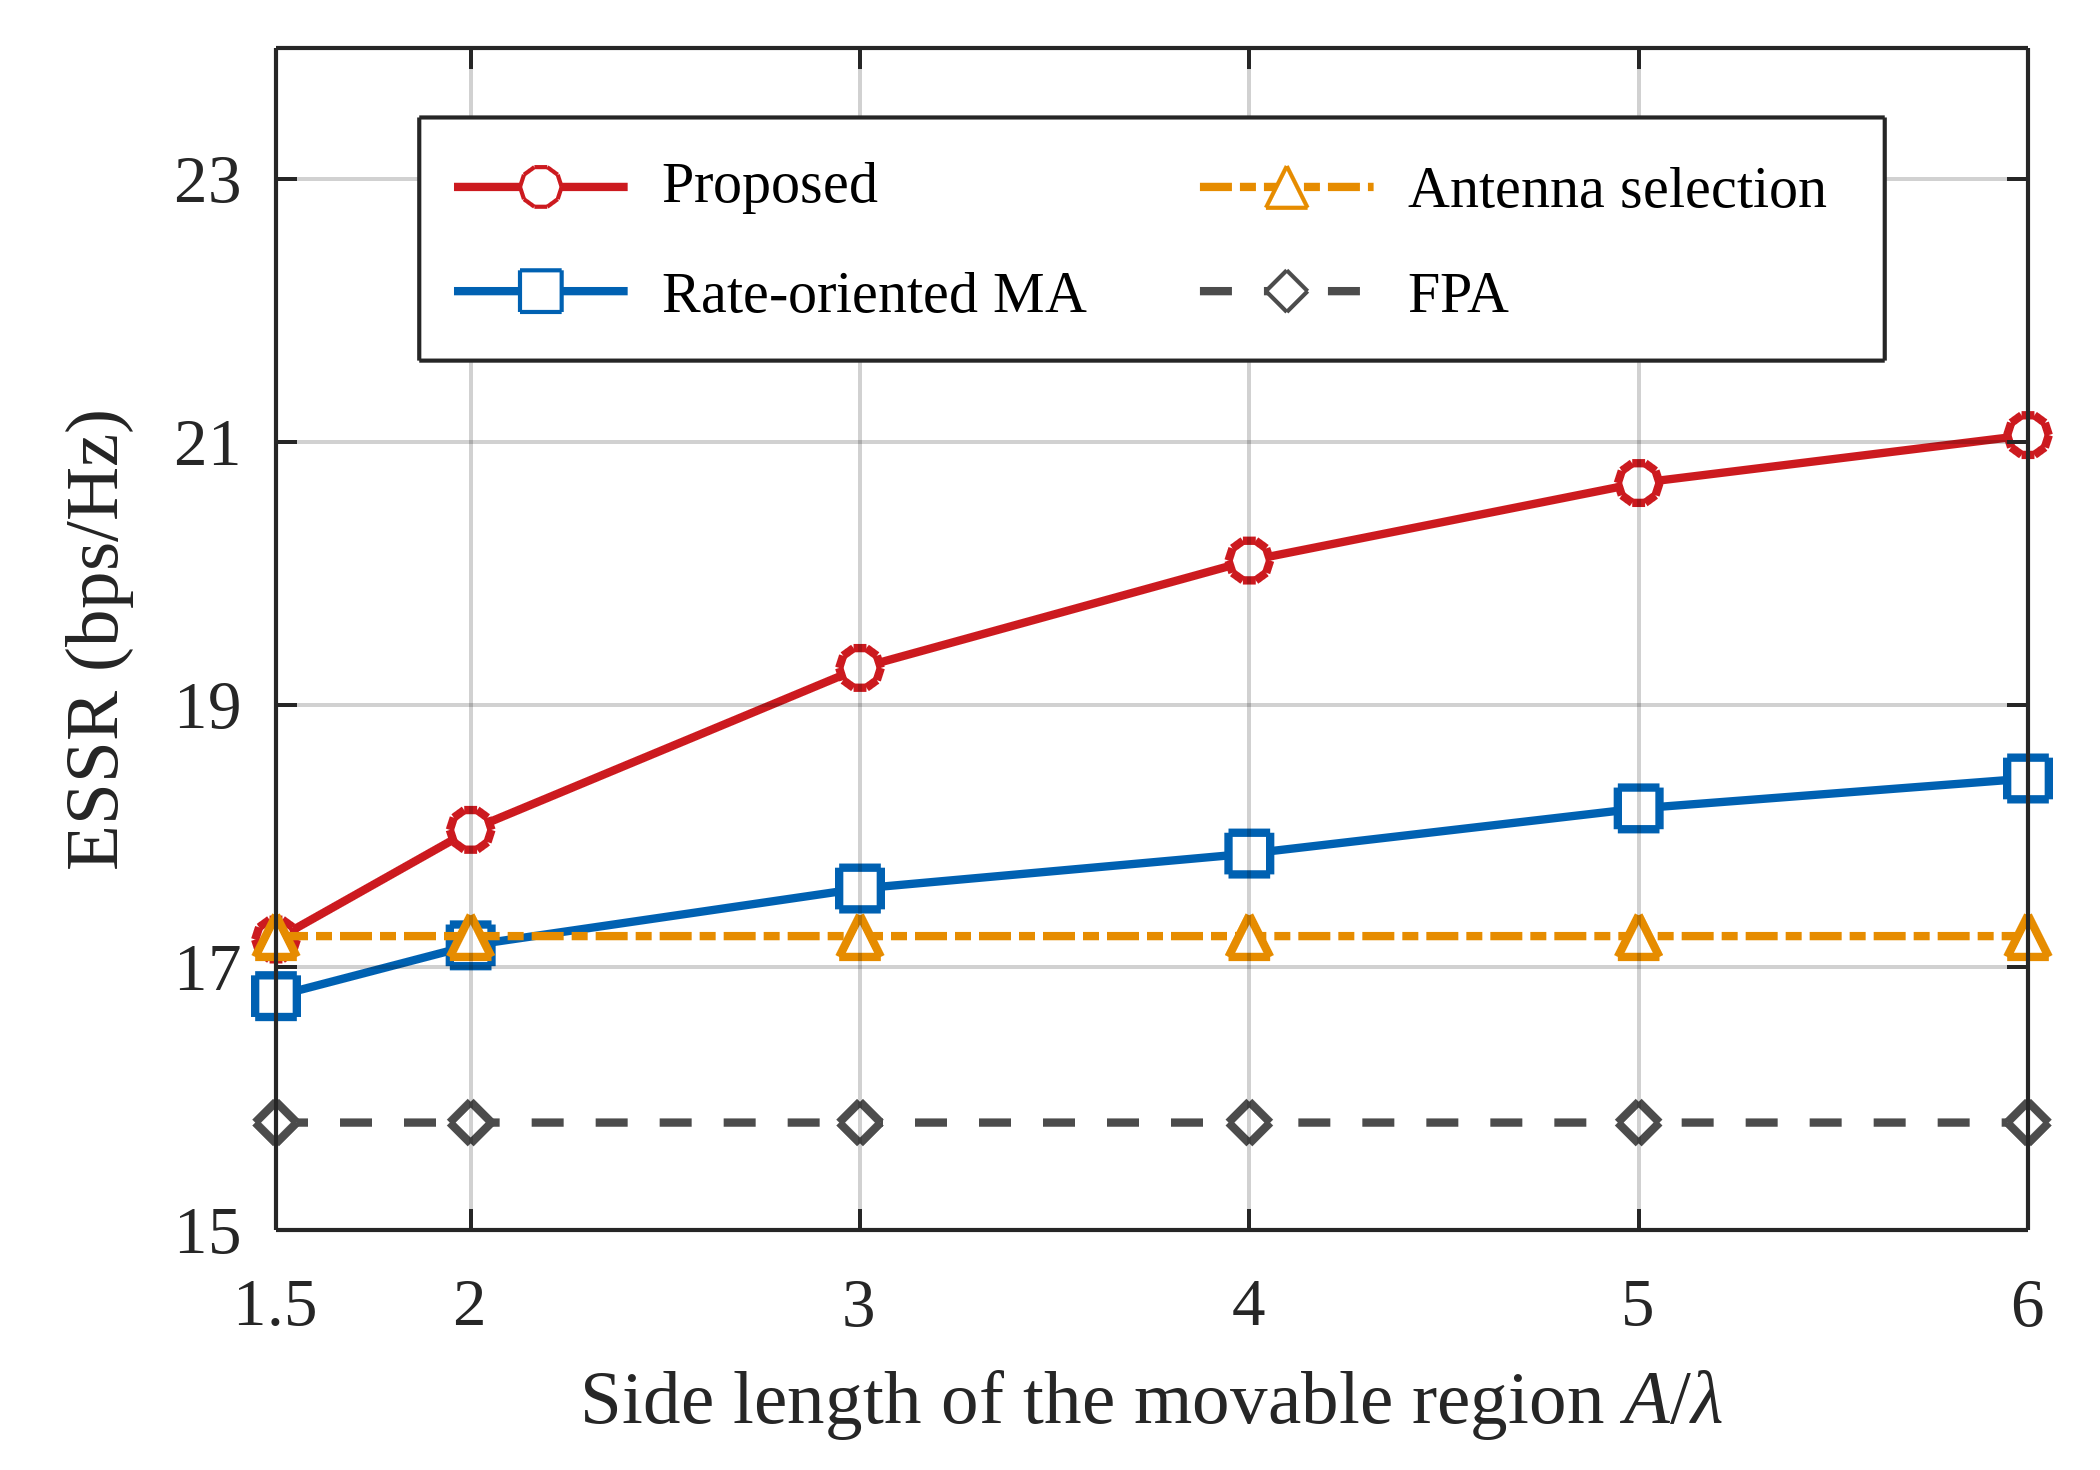
\includegraphics[width=\columnwidth]{fig6_essr_region}
\caption{ESSR versus the side length $A$ of the movable region.}
\label{fig:region}
\end{figure}

Fig.~\ref{fig:region} shows the ESSR versus the side length $A$ of the movable region, where the FPA and AS do not depend on $A$. The ESSR of the proposed design increases with $A$, since a larger region provides more spatial degrees of freedom for decorrelating the LoS components of Eve and the LUs, and its gain over the FPA increases from 8.8\% for $A=1.5\lambda$, where the region is only slightly larger than the footprint of the UPA, to 33.1\% for $A=6\lambda$. In contrast, the rate-oriented MA improves much more slowly with $A$, i.e., the gain over it increases from 2.6\% to 14.2\%, which again shows that the region is exploited for secrecy mainly through Eve-aware positioning. For $A=1.5\lambda$, the candidate array of AS occupies the same region, and AS performs comparably to the proposed design with twice as many antennas, but the gain over AS increases to 22.1\% for $A=6\lambda$. If the $2N$ candidates of AS are instead spread over $\mathcal C$ as a $4\times4$ UPA with spacings $A/3$, AS also exploits the enlarged aperture with the same Eve-aware metric and achieves, e.g., 19.34~bps/Hz for $A=4\lambda$, i.e., Proposition~\ref{prop:eve} also benefits AS-based arrays. Nevertheless, the proposed design still outperforms this AS by 3.7\%--4.3\% for $A\ge3\lambda$ with half the number of antennas and without an RF switching network spanning the region.

The gain of the proposed design also depends on the angular offset $\Delta$ between Eve and LU~1, which we varied from $0.02$ to $0.5$~rad (the curves are omitted for brevity). For $\Delta=0.02$~rad, Eve is almost aligned with LU~1, their LoS components can hardly be decorrelated with an aperture of $4\lambda$, and the proposed design performs within 0.9\% of the rate-oriented MA. As $\Delta$ increases, the gain over the rate-oriented MA increases to 14.4\% at $\Delta=0.2$~rad and then decreases to 10.9\% at $\Delta=0.5$~rad, where Eve becomes separable even with Eve-unaware positions. For a single LU, i.e., $M=1$, the ergodic rate of the LU does not depend on the antenna positions for a given power (Remark~\ref{rem:special}), so that the rate-oriented MA keeps the initial UPA and coincides with the FPA, which is consistent with~\cite{ZhengTCOM2025}. In contrast, for $\Delta=0.1$~rad, the proposed design improves the ergodic secrecy rate from 4.22 to 7.46~bps/Hz, i.e., by 76.6\%, compared with 4.74 and 6.45~bps/Hz for AS and the sparse FPA, by reducing the LoS correlation $|\hb_1^H(\bt)\gb(\bt)|^2$ in~\eqref{eq:c1} and~\eqref{eq:d1}. Accordingly, the optimized AN power fraction decreases from 0.84 for the FPA to 0.51, i.e., the AN-saving effect is even more pronounced for a single LU.

\subsection{Benefit of the Long-Term Power Allocation}\label{sec:sim_pa}

\begin{figure}[t]
\centering
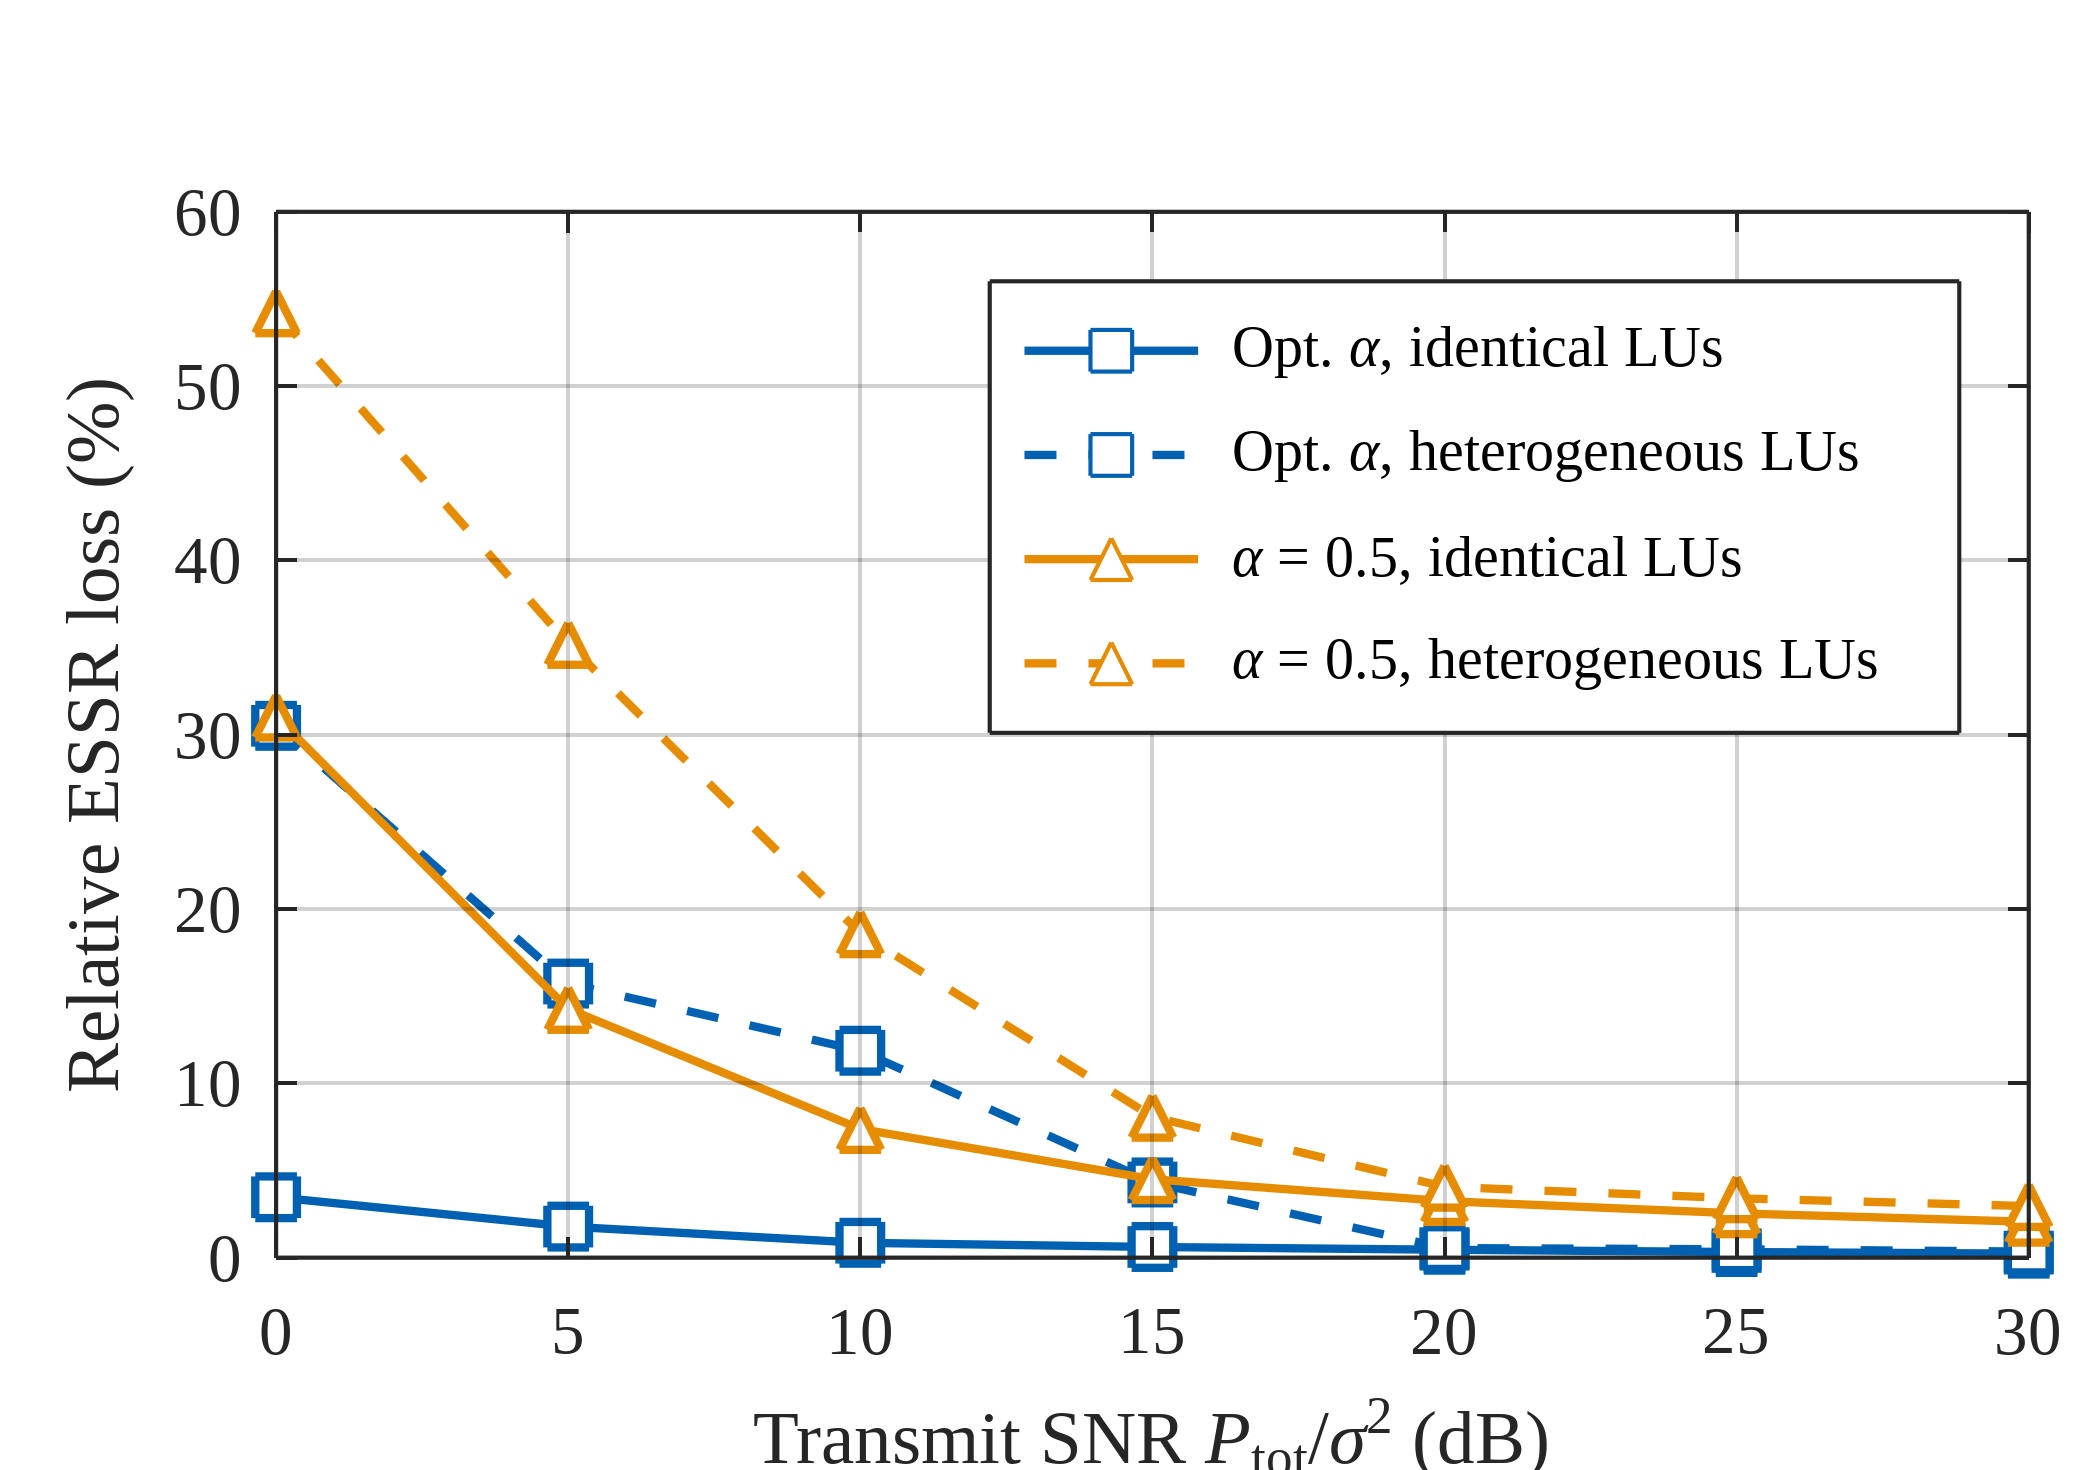
\includegraphics[width=\columnwidth]{fig7_power_allocation}
\caption{Relative ESSR loss $100(1-R_{\mathrm{EP}}/R_{\mathrm{prop}})\%$ of the equal-power (EP) benchmarks w.r.t. the proposed power allocation for identical LUs and heterogeneous LUs with $[\beta_1,\beta_2,\beta_3]=[0,-10,-20]$~dB, where the positions are optimized by Algorithm~\ref{alg:ao} for each power allocation.}
\label{fig:pa}
\end{figure}

Fig.~\ref{fig:pa} compares the proposed power allocation with two benchmarks with equal power among the LUs, i.e., $p_m=\alpha\Ptot/M$ and $q=(1-\alpha)\Ptot/(N-M)$, where $\alpha$ is either optimized by a one-dimensional search, similar to~\cite{Zhou2010}, or fixed to $0.5$, similar to~\cite{ChenArxiv2026}. For all the schemes, the antenna positions are optimized by Algorithm~\ref{alg:ao}, where the objective of the equal-power benchmarks is $\sum_{m=1}^M\tilde R_m^{\mathrm{sec}}$, since the LUs cannot be switched off (cf.\ Proposition~\ref{prop:plus}). For identical LUs as in the previous figures, the equal power allocation with optimized $\alpha$ is nearly optimal, i.e., its ESSR loss is below 1\% for $\Ptot/\sigma^2\ge10$~dB and at most 3.5\%, since the LUs have similar effective channel gains, which are further balanced by the optimized positions, so that the ESSR is mainly determined by the information--AN power splitting (cf.\ Remark~\ref{rem:highsnr}). For heterogeneous LUs, however, the loss is significant at low-to-moderate SNR, e.g., 30.5\% and 11.9\% at $0$ and $10$~dB, respectively, since the proposed power allocation switches off or throttles the LUs whose effective channel gains are comparable to that of Eve (Proposition~\ref{prop:wf}). Further simulations with $[\beta_1,\beta_2,\beta_3]=[0,-\varsigma/2,-\varsigma]$~dB show that this gain becomes significant for $\varsigma\ge10$~dB at $0$~dB and for $\varsigma\ge15$~dB at $10$~dB. As the SNR increases, all the LUs achieve positive secrecy rates, and the loss vanishes, similar to conventional water-filling. Moreover, fixing $\alpha=0.5$ causes an ESSR loss of 2.1\%--31.0\% for identical LUs and 3.0\%--54.2\% for heterogeneous LUs, which is most pronounced at low SNR, where little or no AN is needed. Hence, the information--AN power splitting is the dominant component of the long-term power allocation, whereas the per-user power allocation, which comes at a negligible complexity owing to Proposition~\ref{prop:wf}, is beneficial for heterogeneous LUs at low-to-moderate SNR.

% =============================================================================
\section{Conclusion}\label{sec:conclusion}
% =============================================================================
This paper proposed a two-timescale secure transmission framework for an MA-enabled multiuser downlink system with a passive Eve, where the antenna positions and the long-term power allocation are optimized based on the statistical CSI, and ZF precoding and null-space AN are designed based on the instantaneous CSI of the LUs. We derived a closed-form approximation of the ergodic wiretap rate, which shows that the antenna positions affect the ESSR only through three geometric quantities characterizing the decorrelation among the LUs, the information leakage, and the AN received by Eve, and developed an AO algorithm with secrecy water-filling and MM-based position updates. Numerical results demonstrated that the proposed secrecy-aware positioning outperforms the rate-oriented two-timescale MA design, antenna selection, and FPA arrays, enhances the secrecy performance even for a single LU, and reduces the AN power required for secure transmission, also against an Eve that treats the inter-user interference as noise and under moderate errors in the AoD of Eve. Extending the framework to multiple or multi-antenna eavesdroppers and to imperfect instantaneous CSI of the LUs is an interesting direction for future work.

% =============================================================================
\appendices
\section{Proof of Lemma~\ref{lem:det}}\label{app:det}
% =============================================================================
For brevity, let $\bPhi\triangleq\bPhi_{\bF}$. We first prove~\eqref{eq:lem_c}. Replacing $(\bF^H\bF)^{-1}$ in the unnormalized ZF direction by $\bPhi^{-1}=(\E\{\bF^H\bF\})^{-1}$ yields $\wb_m(\bF)\approx\bF\bPhi^{-1}\be_m/\|\bF\bPhi^{-1}\be_m\|$. Then, we approximate the mean of $|\bb^H\bF\bPhi^{-1}\be_m|^2/\|\bF\bPhi^{-1}\be_m\|^2$ by the ratio of the means of its numerator and denominator, in the same spirit as~\cite[Lemma~1]{ZhangJSTSP2014}. Since $\E\{\bW\}=\mathbf 0$ and $\E\{\bW\mathbf x\mathbf x^H\bW^H\}=\|\mathbf x\|^2\bI_N$ for any deterministic $\mathbf x$, we have
\begin{align}
\E\{|\bb^H\bF\bPhi^{-1}\be_m|^2\}&=|\bb^H\Fb\bPhi^{-1}\be_m|^2+\|\bb\|^2\|\bPhi^{-1}\be_m\|^2\nonumber\\
&=\big|[\bPhi^{-1}\Fb^H\bb]_m\big|^2+\|\bb\|^2[\bPhi^{-2}]_{m,m},\label{eq:app1}\\
\E\{\|\bF\bPhi^{-1}\be_m\|^2\}&=\be_m^T\bPhi^{-1}\bPhi\bPhi^{-1}\be_m=[\bPhi^{-1}]_{m,m},\label{eq:app2}
\end{align}
which lead to~\eqref{eq:lem_c}. Next, we prove~\eqref{eq:lem_d}. Replacing $(\bF^H\bF)^{-1}$ in $\mathbf P_{\bF}\triangleq\bI_N-\mathbf P_{\bF}^\perp=\bF(\bF^H\bF)^{-1}\bF^H$ by $\bPhi^{-1}$ and using $\E\{\bW\bPhi^{-1}\bW^H\}=\tr(\bPhi^{-1})\bI_N$ yield
\begin{equation}\label{eq:app3}
\E\{\mathbf P_{\bF}\}\approx\bPi+\tr(\bPhi^{-1})\bI_N,\qquad\bPi\triangleq\Fb\bPhi^{-1}\Fb^H,
\end{equation}
where $\bPi$ and $\tr(\bPhi^{-1})\bI_N$ represent the parts of the signal subspace induced by the LoS and NLoS components, respectively. However, \eqref{eq:app3} lets the NLoS component capture the same fraction $\tr(\bPhi^{-1})$ of every direction, including those already captured by the LoS component. Hence, it counts the energy of $\bb$ in these directions twice, and $\bb^H(\bI_N-\bPi-\tr(\bPhi^{-1})\bI_N)\bb$ may even become negative when $\bb$ is closely aligned with the column space of $\Fb$. To avoid this double counting, we let the NLoS component capture a fraction $\epsilon\in[0,1]$ of the complement of $\bPi$ only, i.e.,
\begin{equation}\label{eq:app4}
\E\{\mathbf P_{\bF}\}\approx\bPi+\epsilon(\bI_N-\bPi),
\end{equation}
which satisfies $\mathbf 0\preceq\bPi+\epsilon(\bI_N-\bPi)\preceq\bI_N$ since $\mathbf 0\preceq\bPi\prec\bI_N$, as shown below. The fraction $\epsilon$ is determined by the identity $\tr(\mathbf P_{\bF})=k$, which holds for every realization of $\bF$. Since $\tr(\bPi)=\tr\big(\bPhi^{-1}(\bPhi-N\bI_k)\big)=k-N\tr(\bPhi^{-1})$, taking the trace of both sides of~\eqref{eq:app4} yields $k-N\tr(\bPhi^{-1})+\epsilon\big(N-k+N\tr(\bPhi^{-1})\big)=k$, i.e., $\epsilon=N\tr(\bPhi^{-1})/(N-k+N\tr(\bPhi^{-1}))$. Therefore, $\E\{\mathbf P_{\bF}^\perp\}\approx(1-\epsilon)(\bI_N-\bPi)$ with $1-\epsilon=(N-k)/(N-k+N\tr(\bPhi^{-1}))$, which leads to~\eqref{eq:lem_d}.

\textit{Range:} Let $\mu_1,\ldots,\mu_k$ denote the singular values of $\Fb$. The nonzero eigenvalues of $\bPi$ are $\mu_i^2/(\mu_i^2+N)<1$, and thus $\mathbf 0\preceq\bPi\prec\bI_N$. Moreover, $\bPhi\succeq N\bI_k$ implies $0<\tr(\bPhi^{-1})\le k/N$, and thus $1-\epsilon\in[1-k/N,1)$. Hence, the right-hand side of~\eqref{eq:lem_d} lies in $[0,\|\bb\|^2]$. For~\eqref{eq:lem_c}, by the Cauchy--Schwarz inequality, $|[\bPhi^{-1}\Fb^H\bb]_m|^2\le\|\bb\|^2\be_m^T\bPhi^{-1}\Fb^H\Fb\bPhi^{-1}\be_m$, and $\|\bb\|^2[\bPhi^{-2}]_{m,m}\le N\|\bb\|^2[\bPhi^{-2}]_{m,m}$. Since $\be_m^T\bPhi^{-1}(\Fb^H\Fb+N\bI_k)\bPhi^{-1}\be_m=[\bPhi^{-1}]_{m,m}$, the right-hand side of~\eqref{eq:lem_c} lies in $[0,\|\bb\|^2]$.

\textit{Exactness for $\Fb=\mathbf 0$:} In this case, $\bPhi=N\bI_k$ and $\bPi=\mathbf 0$, and the right-hand sides of~\eqref{eq:lem_c} and~\eqref{eq:lem_d} reduce to $\|\bb\|^2/N$ and $\|\bb\|^2(1-k/N)$, respectively. On the other hand, since $\bW$ is unitarily invariant, i.e., $\mathbf Q\bW$ has the same distribution as $\bW$ for any unitary matrix $\mathbf Q$, and $\wb_m(\mathbf Q\bW)=\mathbf Q\wb_m(\bW)$, $\wb_m(\bW)$ is uniformly distributed on the unit sphere, and $\E\{\mathbf P_{\bW}^\perp\}$ commutes with every unitary matrix. Hence, $\E\{|\bb^H\wb_m(\bW)|^2\}=\|\bb\|^2/N$ and $\E\{\mathbf P_{\bW}^\perp\}=(1-k/N)\bI_N$, where the latter follows from $\tr(\mathbf P_{\bW}^\perp)=N-k$.

\textit{Asymptotic exactness for $\Fb=\varrho\Fb_0$:} As $\varrho\to\infty$, $\bF/\varrho\to\Fb_0$ almost surely. Since $\wb_m(\cdot)$ and $\mathbf P_{(\cdot)}^\perp$ are invariant to the scaling of their arguments and continuous at full-column-rank matrices, and $|\bb^H\wb_m(\bF)|^2$ and $\bb^H\mathbf P_{\bF}^\perp\bb$ are bounded by $\|\bb\|^2$, the dominated convergence theorem yields $\E\{|\bb^H\wb_m(\bF)|^2\}\to|\bb^H\wb_m(\Fb_0)|^2$ and $\E\{\bb^H\mathbf P_{\bF}^\perp\bb\}\to\bb^H\mathbf P_{\Fb_0}^\perp\bb$. On the other hand, $\varrho^2\bPhi^{-1}\to(\Fb_0^H\Fb_0)^{-1}$, $\bPi\to\Fb_0(\Fb_0^H\Fb_0)^{-1}\Fb_0^H$, and $\tr(\bPhi^{-1})\to0$. Hence, the right-hand side of~\eqref{eq:lem_d} converges to $\bb^H\mathbf P_{\Fb_0}^\perp\bb$, and that of~\eqref{eq:lem_c} converges to $|[(\Fb_0^H\Fb_0)^{-1}\Fb_0^H\bb]_m|^2/[(\Fb_0^H\Fb_0)^{-1}]_{m,m}=|\bb^H\wb_m(\Fb_0)|^2$, since the second term in the numerator of~\eqref{eq:lem_c} decays as $\mathcal O(\varrho^{-4})$ whereas the denominator decays as $\mathcal O(\varrho^{-2})$. This completes the proof.

% =============================================================================
\section{Derivatives of $\omega_m$, $c_m$, and $d$}\label{app:grad}
% =============================================================================
Let $o_m\triangleq[\bOm^2]_{m,m}$, $\tau\triangleq\tr(\bOm)$, $\tilde{\bv}\triangleq\bOm\bv$, and $\varpi\triangleq\bv^H\bOm\bv$. Since $\bOm$ is Hermitian, \eqref{eq:dOm} can be rewritten as $\dot{\bOm}=-(\bOm\dot{\bl}_n)(\bOm\bl_n)^H-(\bOm\bl_n)(\bOm\dot{\bl}_n)^H$. Hence, the derivatives of $\omega_m$, $o_m$, and $\tau$ w.r.t. $u\in\{x_n,y_n\}$ are given by
\begin{align}
\dot\omega_m&=[\dot{\bOm}]_{m,m}=-2\RE\big\{[\bOm\dot{\bl}_n]_m[\bOm\bl_n]_m^*\big\},\label{eq:a1}\\
\dot o_m&=2\RE\big\{[\bOm\dot{\bOm}]_{m,m}\big\}=-2\RE\big\{[\bOm^2\dot{\bl}_n]_m[\bOm\bl_n]_m^*\nonumber\\
&\qquad\qquad+[\bOm^2\bl_n]_m[\bOm\dot{\bl}_n]_m^*\big\},\label{eq:a2}\\
\dot\tau&=\tr(\dot{\bOm})=-2\RE\big\{\bl_n^H\bOm^2\dot{\bl}_n\big\},\label{eq:a3}
\end{align}
where~\eqref{eq:a2} follows from $[\dot{\bOm}\bOm]_{m,m}=[\bOm\dot{\bOm}]_{m,m}^*$. For $c_m$ in~\eqref{eq:cm}, the derivative of $\tilde{\bv}=\bOm\bv$ is
\begin{equation}\label{eq:a4}
\dot{\tilde{\bv}}=\dot{\bOm}\bv+\bOm\dot{\bv}=-\bOm\dot{\bl}_n\big(\bl_n^H\tilde{\bv}\big)-\bOm\bl_n\big(\dot{\bl}_n^H\tilde{\bv}\big)+\bOm\dot{\bv},
\end{equation}
and thus
\begin{equation}\label{eq:a5}
\dot c_m=\frac{2\RE\big\{[\tilde{\bv}]_m^*[\dot{\tilde{\bv}}]_m\big\}+N\dot o_m-c_m\dot\omega_m}{\omega_m}.
\end{equation}
For $d=(1-\epsilon)(N-\varpi)$ in~\eqref{eq:d}, where $1-\epsilon=(N-M)/(N-M+N\tau)$ as in Appendix~\ref{app:det}, since $\bv^H\dot{\bOm}\bv=-2\RE\{(\tilde{\bv}^H\dot{\bl}_n)(\bl_n^H\tilde{\bv})\}$, we have
\begin{align}
\dot\varpi&=2\RE\{\tilde{\bv}^H\dot{\bv}\}-2\RE\big\{(\tilde{\bv}^H\dot{\bl}_n)(\bl_n^H\tilde{\bv})\big\},\label{eq:a6}\\
\dot d&=-(1-\epsilon)\bigg(\dot\varpi+\frac{N(N-\varpi)\,\dot\tau}{N-M+N\tau}\bigg).\label{eq:a7}
\end{align}
Substituting $\dot\eta_m=-\eta_m\dot\omega_m/\omega_m$, \eqref{eq:a5}, and~\eqref{eq:a7} into~\eqref{eq:dF} yields $\nabla_{\bt_n}F$. All the quantities in~\eqref{eq:a1}--\eqref{eq:a7} are obtained from matrix-vector products with $\bOm$, which require $\mathcal O(M^2)$ operations.

% =============================================================================
\begin{thebibliography}{99}

\bibitem{Wyner1975}
A. D. Wyner, ``The wire-tap channel,'' \emph{Bell Syst. Tech. J.}, vol.~54, no.~8, pp.~1355--1387, Oct. 1975.

\bibitem{Mukherjee2014}
A. Mukherjee, S. A. A. Fakoorian, J. Huang, and A. L. Swindlehurst, ``Principles of physical layer security in multiuser wireless networks: A survey,'' \emph{IEEE Commun. Surveys Tuts.}, vol.~16, no.~3, pp.~1550--1573, 3rd Quart. 2014.

\bibitem{WuJSAC2018}
Y. Wu, A. Khisti, C. Xiao, G. Caire, K.-K. Wong, and X. Gao, ``A survey of physical layer security techniques for 5G wireless networks and challenges ahead,'' \emph{IEEE J. Sel. Areas Commun.}, vol.~36, no.~4, pp.~679--695, Apr. 2018.

\bibitem{Goel2008}
S. Goel and R. Negi, ``Guaranteeing secrecy using artificial noise,'' \emph{IEEE Trans. Wireless Commun.}, vol.~7, no.~6, pp.~2180--2189, Jun. 2008.

\bibitem{Zhou2010}
X. Zhou and M. R. McKay, ``Secure transmission with artificial noise over fading channels: Achievable rate and optimal power allocation,'' \emph{IEEE Trans. Veh. Technol.}, vol.~59, no.~8, pp.~3831--3842, Oct. 2010.

\bibitem{ZhuMag2024}
L. Zhu, W. Ma, and R. Zhang, ``Movable antennas for wireless communication: Opportunities and challenges,'' \emph{IEEE Commun. Mag.}, vol.~62, no.~6, pp.~114--120, Jun. 2024.

\bibitem{ZhuTWC2024Model}
L. Zhu, W. Ma, and R. Zhang, ``Modeling and performance analysis for movable antenna enabled wireless communications,'' \emph{IEEE Trans. Wireless Commun.}, vol.~23, no.~6, pp.~6234--6250, Jun. 2024.

\bibitem{WongTWC2021}
K.-K. Wong, A. Shojaeifard, K.-F. Tong, and Y. Zhang, ``Fluid antenna systems,'' \emph{IEEE Trans. Wireless Commun.}, vol.~20, no.~3, pp.~1950--1962, Mar. 2021.

\bibitem{MaTWC2024}
W. Ma, L. Zhu, and R. Zhang, ``MIMO capacity characterization for movable antenna systems,'' \emph{IEEE Trans. Wireless Commun.}, vol.~23, no.~4, pp.~3392--3407, Apr. 2024.

\bibitem{ZhuTWC2024MU}
L. Zhu, W. Ma, B. Ning, and R. Zhang, ``Movable-antenna enhanced multiuser communication via antenna position optimization,'' \emph{IEEE Trans. Wireless Commun.}, vol.~23, no.~7, pp.~7214--7229, Jul. 2024.

\bibitem{ZhuCL2023}
L. Zhu, W. Ma, and R. Zhang, ``Movable-antenna array enhanced beamforming: Achieving full array gain with null steering,'' \emph{IEEE Commun. Lett.}, vol.~27, no.~12, pp.~3340--3344, Dec. 2023.

\bibitem{HuSPL2024}
G. Hu, Q. Wu, K. Xu, J. Si, and N. Al-Dhahir, ``Secure wireless communication via movable-antenna array,'' \emph{IEEE Signal Process. Lett.}, vol.~31, pp.~516--520, 2024.

\bibitem{HuTMC2024}
G. Hu, Q. Wu, D. Xu, K. Xu, J. Si, Y. Cai, and N. Al-Dhahir, ``Movable antennas-assisted secure transmission without eavesdroppers' instantaneous CSI,'' \emph{IEEE Trans. Mobile Comput.}, vol.~23, no.~12, pp.~14263--14279, Dec. 2024.

\bibitem{XieArxiv2026}
L. Xie, P. Wang, G. Shen, G. Li, W. Mei, and L. Chen, ``Secure communication in MIMOME movable-antenna systems with statistical eavesdropper CSI,'' 2026, \emph{arXiv:2601.14755}.

\bibitem{ChenArxiv2026}
Y. Chen, G. Zhang, M. Cui, H. Fu, Q. Wu, and R. Zhang, ``Sensing-assisted secure communication in MA-aided ISAC: CRB analysis and robust design,'' Apr. 2026, \emph{arXiv:2604.23663}.

\bibitem{ZhengTCOM2025}
Z. Zheng, Q. Wu, W. Chen, and G. Hu, ``Two-timescale design for movable antenna-enabled multiuser MIMO systems,'' \emph{IEEE Trans. Commun.}, vol.~73, no.~11, pp.~10554--10571, Nov. 2025.

\bibitem{HuTVT2025}
G. Hu, Q. Wu, G. Li, D. Xu, K. Xu, J. Si, Y. Cai, and N. Al-Dhahir, ``Two-timescale design for movable antenna array-enabled multiuser uplink communications,'' \emph{IEEE Trans. Veh. Technol.}, vol.~74, no.~3, pp.~5152--5157, Mar. 2025.

\bibitem{ZhaoTWC2021}
M.-M. Zhao, Q. Wu, M.-J. Zhao, and R. Zhang, ``Intelligent reflecting surface enhanced wireless networks: Two-timescale beamforming optimization,'' \emph{IEEE Trans. Wireless Commun.}, vol.~20, no.~1, pp.~2--17, Jan. 2021.

\bibitem{ZhangJSTSP2014}
Q. Zhang, S. Jin, K.-K. Wong, H. Zhu, and M. Matthaiou, ``Power scaling of uplink massive MIMO systems with arbitrary-rank channel means,'' \emph{IEEE J. Sel. Topics Signal Process.}, vol.~8, no.~5, pp.~966--981, Oct. 2014.

\bibitem{ZhuTWC2014}
J. Zhu, R. Schober, and V. K. Bhargava, ``Secure transmission in multicell massive MIMO systems,'' \emph{IEEE Trans. Wireless Commun.}, vol.~13, no.~9, pp.~4766--4781, Sep. 2014.

\bibitem{Gopala2008}
P. K. Gopala, L. Lai, and H. El Gamal, ``On the secrecy capacity of fading channels,'' \emph{IEEE Trans. Inf. Theory}, vol.~54, no.~10, pp.~4687--4698, Oct. 2008.

\bibitem{Horn2013}
R. A. Horn and C. R. Johnson, \emph{Matrix Analysis}, 2nd ed. Cambridge, U.K.: Cambridge Univ. Press, 2013.

\bibitem{Ngo2013}
H. Q. Ngo, E. G. Larsson, and T. L. Marzetta, ``Energy and spectral efficiency of very large multiuser MIMO systems,'' \emph{IEEE Trans. Commun.}, vol.~61, no.~4, pp.~1436--1449, Apr. 2013.

\bibitem{Boyd2004}
S. Boyd and L. Vandenberghe, \emph{Convex Optimization}. Cambridge, U.K.: Cambridge Univ. Press, 2004.

\bibitem{Sun2017}
Y. Sun, P. Babu, and D. P. Palomar, ``Majorization-minimization algorithms in signal processing, communications, and machine learning,'' \emph{IEEE Trans. Signal Process.}, vol.~65, no.~3, pp.~794--816, Feb. 2017.

\bibitem{Beck2017}
A. Beck, \emph{First-Order Methods in Optimization}. Philadelphia, PA, USA: SIAM, 2017.

\end{thebibliography}

\end{document}
